%==============================================================================
% Drop-in Overleaf-ready LaTeX file
% Copy this entire file into Overleaf as a new .tex document, then upload
%   - figures/08_curves_main.png
%   - figures/09_curves_per_class.png
% to the same Overleaf project (or update the \includegraphics paths below).
% (Per-specialty and best-vs-last analyses are reported as tables, not figures,
%  per the constraint that only Figs 8 and 9 are included as graphics.)
%
% Compiles standalone with pdflatex. No external .bib needed — references
% are embedded as a thebibliography block.
%
% Tables added since first draft:
%   - tab:per-specialty   — per-client-pair test F1 with Wilcoxon p
%   - tab:best-vs-last    — peak vs final round val macro-F1
%   - tab:robustness      — centralised baseline, IID, Dirichlet (HPC pending)
%
% PLACEHOLDER SYSTEM (added 2026-05-18, HPC down for ~3 days):
%   - All HPC-pending data is wrapped in \TODOhpc{...} which renders as
%     red [HPC PENDING: …] when \showtodotrue (default on).
%   - The full TODO checklist is in §sec:todo near the end of the document.
%   - To hide all placeholders in a clean compile: \showtodofalse (line ~46).
%   - To find every placeholder:  grep -n "TODOhpc" 09_overleaf_ready.tex
%==============================================================================
\documentclass[11pt,a4paper]{article}

\usepackage[utf8]{inputenc}
\usepackage[T1]{fontenc}
\usepackage{graphicx}
\usepackage{booktabs}
\usepackage{amsmath, amssymb}
\usepackage{microtype}
\usepackage{hyperref}
\usepackage{caption}
\usepackage{xcolor}
\usepackage[margin=2.5cm]{geometry}
\usepackage{setspace}
\usepackage{tikz}
\usetikzlibrary{positioning, shapes.geometric, arrows.meta, fit, backgrounds}
\usepackage{algorithm}
\usepackage{algpseudocode}
\usepackage[authoryear,round]{natbib}
\onehalfspacing

% --- TODO / pending-HPC markers ----------------------------------------------
% These macros make HPC-pending placeholders visible in the compiled PDF.
% Search the source for "TODOhpc" or "PENDING" to find every spot to update
% when results arrive. To hide the markers in the final submitted PDF, set
% the boolean below to false (one toggle disables all markers project-wide).
\newif\ifshowtodo
\showtodotrue   % flip to \showtodofalse before final submission
\newcommand{\TODOhpc}[1]{%
  \ifshowtodo\textcolor{red}{\textbf{[HPC PENDING: #1]}}\else#1\fi}
\newcommand{\PENDING}{\TODOhpc{result}}

\title{Federated Optimisation on DermaMNIST: A Paired-Seed Empirical
Comparison of FedAvg, FedProx, and FedNova Under Statistical and
Computational-Work Heterogeneity}
\author{}
\date{}

\begin{document}
\maketitle

\begin{abstract}
Federated Learning (FL) trains models across data silos without
centralising patient data, but the canonical FedAvg algorithm
\citep{mcmahan2017fedavg} suffers under client heterogeneity. We
evaluate FedProx \citep{li2020fedprox}, which adds a proximal
regulariser to local objectives, on DermaMNIST --- a 7-class
skin-lesion classification dataset with severe class imbalance
(58:1 between majority and minority classes). We design a custom
non-IID partition (\texttt{balanced\_paired\_7\_clients}) in which
every minority class is held by exactly two clients, avoiding the
catastrophic per-class regression observed under singleton-class
partitions. Across 10 paired-seed runs ($R = 150$ rounds, $E = 20$
local epochs, $\mu = 0.01$), FedProx achieves a mean test macro-F1
of $0.508 \pm 0.014$ against FedAvg's $0.481 \pm 0.025$ --- a
within-pair improvement of $\Delta = +0.027 \pm 0.035$ (paired
Wilcoxon $p = 0.020$, rank-biserial $r = +0.818$). FedProx wins on
9 of 10 paired seeds. The largest per-class gain is on melanoma
($\Delta = +0.114$, $p = 0.006$), the most clinically critical
lesion. No class regresses by more than $0.012$ F1, satisfying the
pre-registered safety criterion. FedProx additionally reduces
across-seed variance by 45\%, suggesting more stable convergence
under non-IID conditions.
\end{abstract}

\tableofcontents
\newpage
\listoffigures
\newpage
\listoftables
\newpage

%==============================================================================
\section{Introduction}\label{sec:intro}
%==============================================================================

Skin cancer is one of the most common malignancies worldwide, and
melanoma in particular accounts for the great majority of skin-cancer
deaths despite representing fewer than 5\% of cases. The outcome of a
melanoma diagnosis is exquisitely sensitive to the time at which the
disease is detected: five-year survival rates exceed 99\% when the
lesion is identified while still localised, falling to under 35\% once
the disease has metastasised. This stark survival gradient has
motivated a generation of computer-aided diagnostic systems based on
dermoscopic images, and the recent availability of large-scale
labelled image datasets has made deep learning the de facto
methodology in this space. The HAM10000 collection
\citep{tschandl2018ham10000}, assembled from multiple clinical sites
and comprising 10{,}015 dermoscopic images across seven diagnostic
categories, has become the standard benchmark for this class of
system. The class distribution of HAM10000 --- and of clinical
practice more generally --- is severely imbalanced: melanocytic nevi
(benign moles) account for roughly two-thirds of the recorded cases,
while clinically critical categories such as dermatofibroma and
vascular lesions are each represented by under 2\%. The asymmetry of
clinical cost matches but does not exactly mirror this distribution:
a false negative on the rare melanoma class delays diagnosis of a
lethal disease, while a false positive on a common nevus triggers an
unnecessary but recoverable biopsy. Any deployable dermatology AI
system must therefore demonstrate not only high overall accuracy but
specifically strong recall on the clinically critical minority
classes.

The dataset-driven progress that has powered medical AI is, however,
in tension with the patient-data privacy regimes that govern
healthcare. The European Union's General Data Protection Regulation
(GDPR) classifies medical images as ``special category'' personal data
subject to strict consent and processing constraints; the United
States Health Insurance Portability and Accountability Act (HIPAA)
places equivalent obligations on covered entities. Multi-site clinical
datasets are difficult to assemble in practice: each contributing
institution must navigate its own institutional review board, secure
individual patient consent for secondary research use, anonymise the
source data, and negotiate transfer agreements that frequently forbid
raw-image sharing entirely. Even when such pooling is legally
feasible, the resulting datasets are slow to assemble and rarely
updateable --- by the time the legal-administrative pipeline has
closed, the underlying clinical practice may have moved on. Federated
learning (FL) was introduced by \citet{mcmahan2017fedavg} precisely as
a response to this class of problem. In an FL deployment, each
participating site retains its raw data and trains a local model;
only model parameters or gradient summaries cross the network. A
central server aggregates these summaries, producing a global model
that benefits from the union of the per-site cohorts without any
patient image ever leaving its institution of origin. The
federated-learning literature has expanded substantially in the years
since \citeauthor{mcmahan2017fedavg}'s original proposal
\citep{kairouz2021advances}, with applications now spanning radiology,
histopathology, and ophthalmology; a particularly visible
demonstration of FL deployed in clinical medical imaging is the
multi-institutional brain-tumour segmentation work of
\citet{sheller2020medicalfl}, which trained a single global U-Net
across ten clinical sites without raw-image sharing and reported
performance comparable to a centralised baseline.

Federated learning has, however, exposed a methodological gap of its
own. The canonical algorithm, federated averaging (FedAvg)
\citep{mcmahan2017fedavg}, averages client parameters in proportion
to local dataset size after each communication round. This rule was
shown empirically to perform well when the data distributions held
by different clients are statistically similar, but to degrade ---
sometimes severely --- when those distributions diverge. The pattern,
often referred to as the non-IID degradation problem, has motivated
a family of algorithmic remedies. FedProx \citep{li2020fedprox}
augments each client's local training objective with a proximal
regulariser of the form $(\mu/2)\lVert w - w^t \rVert^2$ that
penalises drift from the round-start global parameter vector,
providing a convergence guarantee for $\gamma$-inexact local updates
and empirically improving on FedAvg under heterogeneous client
distributions. FedNova \citep{wang2020fednova} addresses a
complementary axis of heterogeneity: when clients differ not in their
data but in the amount of local computation they perform per round
(because of hardware diversity, network conditions, or scheduling
constraints), the naïve size-weighted aggregation rule is shown to
be \emph{objective-inconsistent}, and FedNova normalises each
client's update by the effective number of local SGD steps to
correct this bias. Despite the maturity of these three algorithms,
paired-seed empirical comparisons specifically on dermatology
benchmarks are surprisingly thin in the federated-learning
literature. The original FedProx paper validates on Synthetic,
FEMNIST, Shakespeare, and Sentiment140 --- none of them medical;
FedNova validates on CIFAR-10 and similar generic vision benchmarks.
Where federated learning has been applied to medical imaging, the
comparisons typically test FedAvg against a single proximal variant
on a single partition, without the within-pair statistical machinery
that allows the experimentally relevant question --- ``for a given
paired seed, which algorithm produces the better global model?''
--- to be answered with controlled across-seed variance.

This dissertation reports a paired-seed empirical comparison of
FedAvg, FedProx, and FedNova on a federated formulation of the
DermaMNIST classification benchmark, which is the resized
MedMNIST~v2 distribution of HAM10000. The scope is deliberately
bounded. Heterogeneity is simulated: we partition a single dataset
(DermaMNIST) across seven synthetic clients by class index, producing
controlled non-IID conditions of varying severity, but we do not
combine images from independent institutions, scanners, or patient
populations. Hardware heterogeneity is not modelled; what we call
``system heterogeneity'' in the corresponding section is strictly
variable per-client local-step counts, a closely related but
narrower manipulation than the wall-clock heterogeneity of real
deployments. All images are at $28 \times 28$ resolution rather
than the $64 \times 64$ of the source MedMNIST distribution (or the
$600 \times 450$ of the original HAM10000 photographs), a deliberate
compute-economy choice that makes ten paired seeds tractable on a
single A100 GPU within the available HPC budget. Consequently, the
relative algorithmic differences this dissertation reports should be
interpreted as evidence about FedAvg, FedProx, and FedNova under
controlled, simulated heterogeneity at fixed resolution, not as
estimates of clinical performance. The transferability of those
relative differences to higher resolutions, real multi-site
deployments, or alternative dermatology cohorts is an open empirical
question, identified as the primary direction for follow-up work in
\S\ref{sec:future}.

\paragraph{Contributions.} The substantive contributions of this
dissertation are:
\begin{itemize}
\item \textbf{Paired-seed protocol with bit-equivalence at $\mu = 0$.}
We design an experimental protocol in which FedAvg and FedProx share
identical partitions, initial model weights, per-(round, client)
DataLoader random-number generators, dropout masks, and
system-heterogeneity schedules. Bit-equivalence at $\mu = 0$ is
verified by seven unit tests at $10^{-8}$ tolerance over per-round
history, final aggregated state-dictionaries, and test-set metrics.
Within-pair differences therefore reflect only the algorithmic gating
of the proximal term and not any artefact of independent random-number
generators or framework choices.

\item \textbf{A custom \texttt{balanced\_paired\_7\_clients} partition
supporting a clean per-class mechanism prediction.} The partition is
designed so that every minority class is held by exactly two of seven
clients while the majority class (melanocytic nevi) is held by all
seven. The mechanism prediction follows directly: where two clients
hold the same minority class, the proximal regulariser has
consensus-finding work to do; on the universally-held nevi class, it
does not. The dissertation tests this prediction with a per-class
Holm-corrected analysis and a per-specialty contrast.

\item \textbf{Headline empirical result with effect-size and
leave-one-seed-out robustness.} Across ten paired seeds, FedProx
($\mu = 0.01$) improves over FedAvg on test macro-F1 by
$\Delta = +0.027 \pm 0.035$ (paired Wilcoxon $p = 0.020$,
sign-test $p = 0.021$, rank-biserial $r = +0.818$, 9 of 10 paired
wins). The result survives leave-one-seed-out re-testing (all ten
drop-one subsamples remain significant at $\alpha = 0.05$). The
largest per-class gain is on the clinically critical melanoma class
($\Delta = +0.114$, $p_\text{Holm} = 0.041$), the only per-class
result to survive Holm correction across the seven classes.

\item \textbf{Three-regime robustness analysis.} The headline finding
is contextualised by sweeps under three statistical-heterogeneity
regimes: the custom \texttt{balanced\_paired\_7\_clients} partition
(mechanism experiment), a uniform IID null-falsification control
under which FedProx is theoretically predicted to provide no
advantage, and the literature-standard Dirichlet-$\alpha = 0.1$
non-IID partition popularised in the federated-learning benchmarking
literature. The three regimes jointly probe internal validity,
falsifiability, and external validity to a partitioning scheme this
work did not design.

\item \textbf{Independently verified FedNova implementation.} The
FedNova aggregation rule is implemented and verified against
canonical reference values from \citet{wang2020fednova} (e.g.\
$a_i = 41.381$ for $\tau = 10$, $m = 0.9$) via fourteen unit tests
covering the closed-form normaliser, reduction to vanilla SGD at
$m = 0$, monotonicity in $\tau$, sign convention, and reduction to
FedAvg under uniform $\tau$ with zero momentum. The implementation
is used to produce, to our knowledge, the first three-way
(FedAvg vs.\ FedProx vs.\ FedNova) paired-seed comparison on
DermaMNIST.
\end{itemize}

\paragraph{Thesis structure.} \S\ref{sec:background} reviews the
federated-learning problem statement and the mathematical formulation
of FedAvg, FedProx, and FedNova. \S\ref{sec:related} situates this
work against prior federated-optimisation algorithms, non-IID
benchmarks, and federated-learning deployments in medical imaging.
\S\ref{sec:dataset} through \S\ref{sec:metrics} describe the dataset,
the convolutional model, the federated-learning setup, the
algorithmic details, the custom partition, the paired-seed protocol,
and the statistical analysis design. The Results chapter that follows
presents the headline statistical-heterogeneity finding, the
per-class breakdown, the convergence trajectories, the per-specialty
contrast, the peak-versus-final-round analysis, and the
cross-partition robustness study, before consolidating all
heterogeneity conditions into a single summary contrast.  The
Discussion chapter interprets these findings in context.
\S\ref{sec:hardware} documents the compute envelope and the
experiments that were descoped within it. \S\ref{sec:conclusion}
restates the calibrated thesis-level claim and \S\ref{sec:future}
identifies concrete directions for follow-up work.

%==============================================================================
\section{Background}\label{sec:background}
%==============================================================================
This section fixes the federated optimisation problem statement used
throughout the thesis, states the three algorithms under comparison in a
common form, and collects the symbols that subsequent chapters rely on. The
setting is cross-silo \citep{kairouz2021advances}: a small, fixed roster of
trusted clients that all participate in every round, which matches the
deployment scenario of a federation between dermatology departments.

\subsection{Federated learning problem statement}
We are given $K$ clients (in this work $K=7$). Client $i$ holds a private
training set $\mathcal{D}_i$ of size $n_i$, and the union
$\bigcup_i \mathcal{D}_i$ never leaves its origin. The federation learns a
single global model $w \in \mathbb{R}^d$ by minimising a size-weighted average
of the per-client empirical risks,
\begin{equation}
F(w) \;=\; \sum_{i=1}^{K} p_i\, F_i(w),
\qquad
F_i(w) \;=\; \frac{1}{n_i}\!\!\sum_{(x,y)\in\mathcal{D}_i}\!\! \ell\bigl(f_w(x),\, y\bigr),
\qquad
p_i \;=\; \frac{n_i}{\sum_{j=1}^{K} n_j},
\label{eq:fl-objective}
\end{equation}
where $\ell$ is the multi-class cross-entropy loss and $f_w$ is the shared CNN
introduced in \S\ref{sec:model}. Training proceeds in $R$ synchronous
communication rounds. At round $t$ the server broadcasts the current iterate
$w^t$ to a random fraction $C$ of clients (the active subset $S_t$ of size
$\max(1,\lceil C K\rceil)$); each active client runs $E$ local epochs of
mini-batch SGD on $F_i$ to produce $w_i^{t+1}$; the server then aggregates
$\{w_i^{t+1}\}_{i\in S_t}$ into the next iterate $w^{t+1}$. The headline
configuration in this thesis sets $C=1.0$ (full participation), $R=150$, and
$E=20$.

\subsection{The three algorithms}
The three algorithms differ in (i) the local objective the client minimises
and (ii) how the server combines the returned iterates. The local optimiser
(mini-batch SGD with momentum $m=0.9$) and the broadcast schedule are
identical across all three.

\paragraph{FedAvg \citep{mcmahan2017fedavg}.}
Clients minimise $F_i(w)$ directly. The server takes a size-weighted mean of
the returned parameters,
\begin{equation}
w^{t+1} \;=\; \sum_{i\in S_t} p_i\, w_i^{t+1}.
\label{eq:fedavg}
\end{equation}
FedAvg has no explicit defence against client drift: when local objectives
$F_i$ disagree at $w^t$ (the non-IID case), more local steps can move
$w_i^{t+1}$ further from the consensus that minimises $F$.

\paragraph{FedProx \citep{li2020fedprox}.}
Clients minimise a proximally regularised local objective,
\begin{equation}
\widetilde F_i(w;\, w^t) \;=\; F_i(w) \;+\; \frac{\mu}{2}\,\bigl\lVert w - w^t\bigr\rVert_2^2,
\label{eq:fedprox-local}
\end{equation}
which penalises drift from the broadcast anchor $w^t$ with strength controlled
by $\mu \ge 0$. Server aggregation is unchanged from
Equation~\ref{eq:fedavg}. At $\mu = 0$ FedProx reduces exactly to FedAvg; the
headline value in this thesis is $\mu = 0.01$, with a sensitivity sweep over
$\{0.001, 0.01, 0.1, 0.5, 1.0\}$ reported alongside the main results.

\paragraph{FedNova \citep{wang2020fednova}.}
FedNova leaves the local objective at $F_i$ but rescales each client's update
by the L1 norm of its cumulative-momentum series so that clients running
different numbers of local steps $\tau_i$ contribute updates of comparable
magnitude. Writing $d_i = w^t - w_i^{t+1}$ for client $i$'s update,
\begin{equation}
a_i \;=\; \sum_{j=1}^{\tau_i} \frac{1 - m^j}{1 - m}
\;=\; \frac{\tau_i\,(1-m) \;-\; m\,(1-m^{\tau_i})}{(1-m)^2},
\qquad
a_{\mathrm{eff}} \;=\; \sum_{i\in S_t} p_i\, a_i,
\label{eq:fednova-ai}
\end{equation}
\begin{equation}
w^{t+1} \;=\; w^t \;-\; a_{\mathrm{eff}} \,\sum_{i\in S_t} p_i\,\frac{d_i}{a_i}.
\label{eq:fednova-agg}
\end{equation}
When $m=0$ this collapses to $a_i = \tau_i$ (the original FedNova proposal);
when in addition all $\tau_i$ are equal it collapses to FedAvg. FedNova
therefore isolates the heterogeneous-local-work effect that proximal
regularisation does not address directly, making it the canonical comparator
for the system-heterogeneity arm of this study.

\subsection{Notation}
Table~\ref{tab:notation} collects the symbols used throughout the thesis.
The same symbols are reused in the results chapter without redefinition.

\begin{table}[h]
\centering
\small
\caption{Notation used throughout the thesis.}
\label{tab:notation}
\begin{tabular}{l p{0.72\textwidth}}
\toprule
Symbol & Meaning \\
\midrule
$K$               & Number of FL clients (this work: $K=7$). \\
$\mathcal{D}_i$   & Local training dataset held by client $i$. \\
$n_i$             & Number of training samples at client $i$. \\
$p_i$             & Size weight, $p_i = n_i / \sum_{j} n_j$. \\
$F$               & Global objective $F(w) = \sum_i p_i F_i(w)$. \\
$F_i$             & Local empirical risk at client $i$. \\
$w^t$             & Global model parameters at the start of round $t$. \\
$w_i^{t+1}$       & Local parameters returned by client $i$ after round $t$. \\
$R$               & Number of communication rounds (this work: $R=150$). \\
$E$               & Number of local epochs per round (this work: $E=20$). \\
$C$               & Fraction of clients sampled per round (this work: $C=1.0$). \\
$\mu$             & FedProx proximal coefficient (headline: $\mu=0.01$). \\
$\tau_i$          & Number of local SGD steps performed by client $i$ in one round. \\
$a_i$             & FedNova momentum-aware normaliser, Equation~\ref{eq:fednova-ai}. \\
$\Delta$          & Within-pair gap $\Delta = \mathrm{macro\text{-}F1}_{\mathrm{FedProx}} - \mathrm{macro\text{-}F1}_{\mathrm{FedAvg}}$. \\
$r_{rb}$          & Rank-biserial correlation \citep{kerby2014rankbiserial}, the paired-test effect size. \\
\bottomrule
\end{tabular}
\end{table}

\subsection{Hypotheses}\label{sec:hypotheses}
The empirical study tests two pre-registered hypotheses and reports two
auxiliary predictions that act as falsification probes. Pre-registration here
means the hypotheses, partition, and statistical tests were fixed before the
HPC sweeps were submitted; only the test statistics and effect sizes were
re-derived from the run logs.

\paragraph{H1 (within-condition).}
\emph{On the \texttt{balanced\_paired\_7\_clients} partition at $E=20$,
$R=150$, and $\mu=0.01$, FedProx improves test macro-F1 over FedAvg in a
paired-seed comparison.} Operationally: let
$\Delta^{(s)} = \mathrm{macro\text{-}F1}_{\mathrm{FedProx}}^{(s)} - \mathrm{macro\text{-}F1}_{\mathrm{FedAvg}}^{(s)}$
for paired seed $s \in \{1,\dots,10\}$. We test
$H_0\!:\, \mathrm{median}(\Delta) = 0$ against
$H_1\!:\, \mathrm{median}(\Delta) \ne 0$ using the two-sided paired Wilcoxon
signed-rank test at $\alpha = 0.05$ with $n = 10$ seeds, supported by a paired
sign test and the Hodges--Lehmann estimator of $\mathrm{median}(\Delta)$.

\paragraph{H2 (between-condition).}
\emph{Under computational-work heterogeneity (random stragglers, condition
C2), the FedProx-over-FedAvg gap widens relative to the C0 baseline.}
Operationally: per seed $s$, compute $\Delta_{C2}^{(s)}$ and
$\Delta_{C0}^{(s)}$; then test
$H_0\!:\, \mathrm{median}(\Delta_{C2} - \Delta_{C0}) = 0$ via paired Wilcoxon
at a Bonferroni-corrected threshold of $\alpha/2 = 0.025$ (the family covers
both C1 and C2, although only C2 is the primary inferential test; C1 is
reported descriptively because of the documented partition-confound between
fixed-straggler identity and the class mechanism).

\paragraph{Falsification prediction (IID).}
On the IID partition every client sees an i.i.d.\ draw from the same
distribution, so the local objectives $F_i$ agree at every $w^t$ and the
proximal anchor in Equation~\ref{eq:fedprox-local} has nothing to anchor
\emph{to}. We therefore predict $\Delta \approx 0$ and a non-significant
Wilcoxon $p$-value ($p > 0.05$) on IID. A significant positive $\Delta$ under
IID would falsify the drift-control mechanism story and indicate that the
observed headline gap is driven by something other than statistical
heterogeneity.

\paragraph{External-validity prediction (Dirichlet $\alpha = 0.1$).}
Dirichlet partitioning \citep{hsu2019dirichlet} is the field-standard
synthetic non-IID benchmark and is not engineered to maximise the FedProx
advantage in the way \texttt{balanced\_paired\_7\_clients} is. We predict
$\Delta > 0$ on Dirichlet $\alpha = 0.1$ (the result transfers) but with
magnitude $\lvert\Delta_{\mathrm{Dir}}\rvert < \lvert\Delta_{\mathrm{paired}}\rvert$
(the engineered partition still produces the largest effect).

\subsection{Specialist-partition pre-registration}\label{sec:hyp-specialist}
\paragraph{Motivation.}
The headline partition \texttt{balanced\_paired\_7\_clients} holds every
minority class on exactly two clients. The two clients holding the same
class drift in different directions during local SGD, and the FedProx
proximal anchor $(\mu/2)\lVert w - w^t\rVert_2^2$ pulls them back together
at aggregation. This is the regime where the proximal anchor has the
most to anchor against; an examiner can argue the +0.027 macro-F1
advantage is therefore an artefact of the pairing structure rather than
evidence of a general FedProx benefit under label skew. We pre-register
a sister sweep that flips the pairing lever while holding every other
confound constant.

\paragraph{Design.}
The sister partition \texttt{specialist\_7\_clients} (added to
\texttt{mnist\_dermnist/data/partition.py} as
\texttt{SPECIALIST\_7\_CLIENTS\_SPEC}, committed at SHA \texttt{5aba7ad} on
2026-05-21) assigns every minority class to exactly \emph{one} client and
distributes \texttt{nevi} across the six specialty clients in unequal
shares chosen so that the per-client $n_i$ matches
\texttt{balanced\_paired\_7\_clients} exactly:
\{964, 963, 1095, 1094, 1110, 1108, 673\}. Everything else is held
constant: 10 paired seeds, 7 clients, $C=1.0$, $R=150$, $E=20$,
$\mu=0.01$, identical model + optimiser + Flower runtime + test-at-best-
val protocol. The contrast $\Delta_{\mathrm{specialist}}$ vs
$\Delta_{\mathrm{paired}}$ therefore isolates the pairing structure from
quantity-skew, client-count, or global class-composition confounds.

\paragraph{Pre-registered prediction.}
We predict $\Delta_{\mathrm{specialist}} > 0$ \emph{and}
$\lvert\Delta_{\mathrm{specialist}}\rvert < \lvert\Delta_{\mathrm{paired}}\rvert$
on macro-F1. Mechanism: the proximal anchor still damps individual-client
drift relative to the global model under specialist heterogeneity, but
the effect is smaller without paired co-trained drifting clients for the
anchor to reconcile.

\paragraph{Interpretation of every possible outcome.}
\begin{itemize}
  \item $\Delta_{\mathrm{specialist}} \approx \Delta_{\mathrm{paired}}$ —
    the pairing-mechanism story is wrong; the FedProx advantage is a more
    general label-skew regularisation effect (likely implicit
    learning-rate shrinkage on noisy updates). The headline claim must
    be reframed as ``FedProx helps under label skew,'' without the
    paired-drift causal narrative.
  \item $\Delta_{\mathrm{specialist}} > 0$ but smaller in magnitude than
    $\Delta_{\mathrm{paired}}$ — the mechanism story holds: specialist
    drift is also controlled but pairing amplifies the gap. This is the
    pre-registered outcome and the thesis stands as written.
  \item $\Delta_{\mathrm{specialist}} \approx 0$ — FedProx's advantage
    is specifically a co-trained-pair phenomenon; the thesis claim must
    narrow to ``FedProx helps when clients holding the same minority
    class drift apart'' rather than the broader ``FedProx helps under
    label skew.''
  \item $\Delta_{\mathrm{specialist}} < 0$ — unexpected. Report
    honestly and discuss whether specialist heterogeneity creates a
    regime where the proximal anchor harms learning, e.g.\ by over-
    constraining clients whose local objective lies far from the global
    consensus.
\end{itemize}

\paragraph{Inference.}
Same paired Wilcoxon protocol as H1 ($n=10$ paired seeds, two-sided
$\alpha = 0.05$). Effect size: Hodges--Lehmann estimator of
median$(\Delta_{\mathrm{specialist}})$ with the \emph{exact} Walsh-
average-inversion confidence interval at $\alpha = 0.05$
(\emph{not} bootstrap; for $n=10$ the bounds are the 9th smallest and
9th largest of the 55 Walsh averages). Magnitude comparison against
$\Delta_{\mathrm{paired}}$ is descriptive: both effect sizes are reported
with their HL point estimates and exact CIs and the reader is invited to
make the magnitude judgement. Pre-written discussion paragraphs for each
of the four outcomes above are kept in
\texttt{mnist\_dermnist/results/thesis\_ready/writing/specialist\_partition\_scenarios.tex}
so the eventual write-up does not get retro-fitted around the observed
direction. Analysis script:
\texttt{mnist\_dermnist/results/thesis\_ready/scripts/analyse\_specialist\_partition.py}.
Submission script: \texttt{mnist\_dermnist/scripts/submit\_specialist\_partition.sh}
(20 jobs, $\approx$25 GPU-h on A100).

%==============================================================================
\section{Related Work}\label{sec:related}
%==============================================================================
Three streams of work bear directly on the empirical comparison this thesis
performs: the federated optimisation algorithms that the thesis evaluates, the
non-IID benchmarks that establish how such algorithms are stress-tested, and
the medical-imaging FL literature that motivates the use case. This section
reviews each in turn, identifies the gap this thesis addresses, and contrasts
the present contribution against the closest published references.

\subsection{Federated optimisation algorithms}
\label{sec:rw-algorithms}

\paragraph{FedAvg and the client-drift problem.}
The defining algorithm of federated learning is FedAvg
\citep{mcmahan2017fedavg}, which alternates $E$ local SGD epochs at each
client with a size-weighted server average of the returned parameters
(Equation~\ref{eq:fedavg}). The original analysis observed strong empirical
performance on partitions where client data is drawn IID from a single
distribution, and subsequent theory has shown that under IID conditions and
sufficiently small local steps FedAvg converges at the same asymptotic rate
as centralised SGD up to a slowdown that depends on $E$ and the participation
fraction $C$. The intuition is straightforward: with IID local data, each
local SGD step is an unbiased estimator of the global gradient
$\nabla F(w^t)$, so the size-weighted average of local updates is itself an
unbiased estimator and the algorithm inherits centralised SGD's convergence
guarantees up to constants. The failure mode that motivates everything that
follows is the non-IID setting: when local datasets $\mathcal{D}_i$ are drawn
from different distributions the local objectives $F_i$ disagree at every
$w^t$, and more local steps move each $w_i^{t+1}$ further along its own
per-client gradient trajectory rather than the global one. Formally,
$\mathbb{E}\!\left[\nabla F_i(w^t)\right] \ne \nabla F(w^t)$ in general, so
the local update bias accumulates over $E$ epochs. The size-weighted average
of these divergent iterates is not in general a descent step for $F$, and
convergence slows --- or, in extreme cases, fails altogether.
\citet{hsieh2020quagmire} quantify how severe this degradation can be on
practical workloads, with reported accuracy losses of $10$--$50$ percentage
points relative to centralised baselines on image and language tasks, and
introduce the now-standard vocabulary of ``the non-IID quagmire'' under
which subsequent benchmarks are framed.

\paragraph{Three families of remedies.}
The literature has converged on three architectural families of solutions,
each modifying a different part of the FedAvg round.
\emph{(i) Proximal regularisation.} FedProx \citep{li2020fedprox} adds a
quadratic anchor $(\mu/2)\lVert w - w^t\rVert_2^2$ to the local objective
(Equation~\ref{eq:fedprox-local}). The anchor penalises drift from the
broadcast point and yields a $\gamma$-inexact-update convergence framework
under a bounded-dissimilarity assumption
$\lVert \nabla F_i(w) \rVert^2 \le B^2 \lVert \nabla F(w) \rVert^2$ for some
constant $B$; under this assumption \citet{li2020fedprox} prove $O(1/T)$
convergence on non-convex objectives even when clients perform variable
amounts of local work. Empirically, FedProx improves non-IID performance at
the cost of a single new hyperparameter $\mu$, and degrades gracefully:
choosing $\mu$ too small recovers FedAvg, while choosing $\mu$ too large
slows convergence by over-anchoring to a possibly suboptimal $w^t$. The
sweet spot is dataset- and partition-dependent. This thesis evaluates FedProx
in the headline at $\mu = 0.01$ with a sensitivity sweep over
$\mu \in \{0.001, 0.01, 0.1, 0.5, 1.0\}$ to characterise the FedProx-over-
FedAvg gap's robustness to that choice.
\emph{(ii) Control variates.} SCAFFOLD \citep{karimireddy2020scaffold}
maintains client-side and server-side control variates $c_i$ and $c$ that
explicitly correct for client-drift gradient differences. The local update
rule becomes $w \leftarrow w - \eta_l (\nabla F_i(w) - c_i + c)$, where the
$-c_i + c$ term is a variance-reduction control variate that cancels in
expectation under IID data but corrects the per-client gradient bias under
non-IID data. The method enjoys variance-reduction guarantees that are
tighter than FedProx's and matches centralised SGD's asymptotic rate under
arbitrary heterogeneity. The price is twofold: the per-round communication
doubles, because both the parameter update and the control-variate update
must be transmitted, and each client must maintain persistent state across
rounds, which complicates cross-device deployment where clients may drop in
and out. This thesis does \emph{not} evaluate SCAFFOLD: the 2$\times$
communication penalty changes the cost structure of the round, and a fair
comparison would require either equal-communication or equal-rounds
baselines that compare on a different axis from the one the thesis isolates.
\emph{(iii) Aggregation normalisation.} FedNova \citep{wang2020fednova}
leaves the local objective at $F_i$ but rescales each client's returned
update by the L1 norm of its cumulative-momentum series
(Equation~\ref{eq:fednova-ai}). The motivation is the
\emph{objective-inconsistency} problem: when clients run different numbers
of local steps $\tau_i$, the size-weighted FedAvg aggregator implicitly
optimises a perturbed objective $\sum_i p_i \tau_i F_i / \sum_j p_j \tau_j$
rather than the intended $\sum_i p_i F_i$, so clients doing fewer steps
contribute disproportionately small updates and the global iterate drifts
toward the objective of clients doing more. FedNova's per-client
$a_i$-rescaling removes this bias. In the $m=0$, equal-$\tau$ limit FedNova
reduces to FedAvg; in the $m=0$, variable-$\tau$ regime it reduces to the
earlier FedNova-SGD variant; only the momentum case $m > 0$ produces the
full closed-form $a_i$ used here. FedNova is the canonical comparator for
heterogeneous-local-work conditions, and this thesis evaluates it as the
third arm of the system-heterogeneity comparison.

\paragraph{Server-side adaptive optimisers.}
A complementary line of work modifies the \emph{server-side} aggregation rule
rather than the local objective. \citet{reddi2021adaptive} replace the size-
weighted average with adaptive moment estimation (FedAdam, FedYogi, FedAdagrad),
treating client deltas as pseudo-gradients into a server-side optimiser. The
resulting algorithms address slow convergence on heterogeneous data without
modifying the client at all, which is attractive when client compute is
constrained or when the federation includes resource-asymmetric devices.
This thesis does not evaluate the FedAdam family: a clean comparison would
require carefully controlling the server-side learning-rate schedule across
algorithms, and the proximal-vs-normalisation contrast that the thesis
isolates is sharper without that additional axis. Adaptive aggregation is
flagged as future work (\S\ref{sec:future}).

\paragraph{Scope of the present thesis.}
In summary, of the four families above --- FedAvg, proximal regularisation,
control variates, aggregation normalisation, and server-side adaptive
optimisation --- this thesis evaluates three (FedAvg, FedProx, FedNova) and
explicitly scopes out SCAFFOLD (communication asymmetry) and the FedAdam
family (server-side axis). The three algorithms it does evaluate are the
minimum set that lets the thesis attribute observed gaps to specific
mechanisms: FedAvg as the no-intervention baseline, FedProx as the proximal-
anchor mechanism, and FedNova as the aggregation-normalisation mechanism.

\subsection{Non-IID federated learning benchmarks}
\label{sec:rw-benchmarks}

\paragraph{Dirichlet partitioning.}
The most widely adopted protocol for simulating non-IID label skew is the
Dirichlet partitioning scheme of \citet{hsu2019dirichlet}. For each class
$c \in \{1,\dots,C\}$ a vector
$\bm{q}_c \sim \mathrm{Dir}_K(\alpha\bm{1})$ is sampled and class-$c$ samples
are then allocated to the $K$ clients in proportions $q_{c,1}, \dots, q_{c,K}$.
The concentration parameter $\alpha$ controls heterogeneity: small $\alpha$
(e.g.\ $0.1$) yields highly skewed partitions in which each client holds only
a few classes, while large $\alpha$ (e.g.\ $10$ or larger) approximates the
IID limit. In the limit $\alpha \to 0$ each class is concentrated on a
single client (the extreme pathological non-IID case), and in the limit
$\alpha \to \infty$ the partition converges to uniform-IID. The scheme is
attractive because it generates a smooth one-parameter family of partitions
and exposes the algorithm's robustness profile as $\alpha$ varies, but it has
two well-documented limitations: the per-class sampling can produce empty-
client classes that need to be re-rolled, and the resulting per-client
quantities $n_i$ are themselves random, which couples label skew with
quantity skew unless explicit re-balancing is applied. This thesis evaluates
Dirichlet $\alpha = 0.1$ as the external-validity probe alongside the
engineered \texttt{balanced\_paired} partition described in
\S\ref{sec:partition}, with the same seed-fixing protocol so per-seed
Dirichlet draws are reproducible.

\paragraph{NIID-Bench.}
The canonical multi-algorithm comparison on non-IID data is NIID-Bench
\citep{li2022niidbench}, which benchmarks seven federated algorithms across
nine datasets and six non-IID partitioning protocols. The paper's central
empirical finding is that no single algorithm wins uniformly: relative
ordering between FedAvg, FedProx, FedNova, and SCAFFOLD changes as the
heterogeneity axis, the dataset, and the model family change. The
partitioning protocols themselves --- label-quantity (each client gets $k$
of $C$ classes), label-distribution (Dirichlet), feature-distribution (per-
client noise), quantity-skew, and homogeneous (IID) --- formalise the
heterogeneity axes that earlier work surveyed informally and have become
de facto standards in subsequent comparisons. NIID-Bench also documents
that even within a single partition setting the relative ordering can flip
across random seeds, which motivates the paired-seed inferential protocol
this thesis adopts. The NIID-Bench DermaMNIST entry specifically reports
overlapping confidence intervals between FedAvg and FedProx, leaving the
question of whether the difference is statistically significant unanswered:
this thesis fills exactly that gap, with a paired Wilcoxon at $n=10$ seeds
on the engineered \texttt{balanced\_paired} partition that maximises the
label-skew axis NIID-Bench identified as most sensitive for this dataset.

\paragraph{Taxonomy of heterogeneity axes.}
\citet{kairouz2021advances} provide the field-standard taxonomy of non-IID
data, distinguishing four axes: \emph{label skew} (different clients have
different class priors $p_i(y)$, the dominant axis in cross-silo medical FL
where each site sees a different patient-population case mix),
\emph{feature skew} (the conditional input distribution $p(x \mid y)$
differs across clients, e.g.\ scanner-dependent acquisition protocols
producing systematically different intensity histograms for the same
underlying tissue), \emph{quantity skew} (clients have different $n_i$,
which on its own is a benign axis handled by the size weights $p_i$ but
which interacts multiplicatively with label and feature skew), and
\emph{concept drift} (the label function $p(y \mid x)$ itself differs
across sites or over time, e.g.\ when diagnostic conventions or labelling
guidelines change between institutions). Different algorithmic interventions address different
axes: FedProx and SCAFFOLD primarily target label skew via drift control;
FedBN \citep{li2021fedbn} targets feature skew by keeping batch-norm
statistics local; quantity skew is implicitly handled by the size weights
$p_i$ but interacts with all of the above. This thesis isolates \emph{label
skew} with mild quantity skew: every client in \texttt{balanced\_paired}
holds a distinct class subset (label skew), and the partition slightly
varies $n_i$ across clients (quantity skew), but the dataset is a single
homogeneous source (no feature skew or concept drift). Isolating label skew
this cleanly makes any FedProx advantage attributable to the drift-control
mechanism rather than confounded with feature-shift remedies.

\subsection{Federated learning in medical imaging}
\label{sec:rw-medicalfl}

\paragraph{Foundational work.}
The first widely cited demonstration that federated learning matches
centralised training on a clinically meaningful task is
\citet{sheller2020medicalfl}, which trains a brain-tumour segmentation
model across ten institutions on the BraTS dataset and shows that the
federated model achieves segmentation Dice within $\sim$1\% of a centrally
trained model with the same architecture. Crucially, the study also
compares against single-institution baselines and finds that the federated
model substantially outperforms any individual site, quantifying the
collaborative gain for the first time on real clinical data. The result
established that the privacy-utility trade-off in medical imaging need not
be punitive when inter-site heterogeneity is moderate.
\citet{rieke2020future} provide the broader vision-piece for the field,
surveying the technical, regulatory, and clinical considerations that
distinguish medical FL from FL on consumer devices. They emphasise three
practical constraints absent in the canonical FL formulation: regulatory
heterogeneity across jurisdictions (HIPAA, GDPR, MDR), the need for audit
trails that survive aggregation, and the fact that medical clients are
small in number ($K$ in tens) but rich in data per client, the inverse of
the cross-device profile FedAvg was designed for. They argue that cross-
silo FL between trusted institutions is the most tractable setting for
early deployment, a framing this thesis adopts.

\paragraph{Production-scale medical FL.}
The FeTS study \citep{pati2022fets} brings federated learning to production
scale: 71 sites across six continents collaborate on glioblastoma boundary
detection in a federation that runs over six months, with no central pooling
of patient data at any stage. The paper reports a measurable improvement in
generalisation when the federation includes geographically and demographically
diverse sites, and is the strongest available evidence that the
small-scale findings of \citet{sheller2020medicalfl} extrapolate to
real-world deployment. FeTS used FedAvg with carefully tuned local epochs
rather than any of the heterogeneity-aware algorithms reviewed in
\S\ref{sec:rw-algorithms}; whether FedProx or FedNova would have improved
upon their results remains an open question, and is part of the practical
motivation for studies of the present kind.

\paragraph{Feature-shift remedies.}
A distinct concern in multi-scanner medical imaging is feature shift: even
when the underlying condition is held constant, scanner-specific intensity
distributions and acquisition protocols produce $p(x \mid y)$ that varies
across sites. The standard FL aggregation rule averages batch-norm running
statistics across clients, which propagates each site's idiosyncratic
intensity distribution into a shared estimator that fits none of them well.
FedBN \citep{li2021fedbn} addresses this by keeping batch-normalisation
statistics --- both the running mean and variance buffers and the affine
$\gamma, \beta$ parameters --- \emph{local} (i.e.\ never aggregated) while
sharing all other convolutional and linear parameters; on multi-scanner MRI
and X-ray cohorts the intervention recovers most of the gap between
federated and centralised performance, and incurs no extra communication
because the local parameters are never transmitted. This thesis does not
evaluate FedBN: DermaMNIST is a single homogeneous source with no scanner
axis, so feature shift is absent by construction, and the CNN used here
employs GroupNorm \citep{wu2018groupnorm} rather than BatchNorm precisely
to side-step the FedBN-style aggregation question. FedBN is nonetheless
relevant context: it shows that the right algorithmic intervention depends
on which heterogeneity axis dominates in the deployment setting, which is
a recurring theme of \S\ref{sec:rw-algorithms} and
\S\ref{sec:rw-benchmarks}.

\paragraph{Where this thesis fits.}
The literature surveyed above leaves a specific empirical gap that this
thesis fills. NIID-Bench compares algorithms across many datasets but
without a paired-seed inferential protocol, leaving DermaMNIST's
FedAvg-vs-FedProx ordering statistically unresolved. The medical-FL line
(\citealt{sheller2020medicalfl, rieke2020future, pati2022fets}) provides
deployment evidence under FedAvg but does not isolate algorithmic
interventions. The present thesis combines the contributions absent
from each individual line: \emph{(a)} a strict paired-seed protocol with
formal Wilcoxon inference on DermaMNIST classification, \emph{(b)} the
addition of FedNova as the heterogeneous-computation arm so the
proximal-vs-normalisation contrast can be tested directly, and \emph{(c)}
explicit C0/C1/C2 conditions that decouple statistical heterogeneity
(non-IID label skew) from computational-work heterogeneity (random
stragglers). The novelty is not the algorithms or the dataset; it is the
combination, and the inferential discipline imposed on top.

%==============================================================================
\section{Experimental Setting}
%==============================================================================

Figure~\ref{fig:pipeline} summarises the end-to-end pipeline. The
remainder of this section describes each stage in detail: the dataset
(\S\ref{sec:dataset}), the convolutional model (\S\ref{sec:model}),
the federated training setup (\S\ref{sec:fl-setup}), the
two algorithms and the proximal-term gating that ensures
$\mu = 0$ bit-equivalence with FedAvg (\S\ref{sec:algorithms}), the
custom partition that supports the per-class mechanism prediction
(\S\ref{sec:partition}), the paired-seed reproducibility protocol
(\S\ref{sec:protocol}), and the evaluation metrics together with the
statistical-inference design (\S\ref{sec:metrics}).

\begin{figure}[!htbp]
\centering
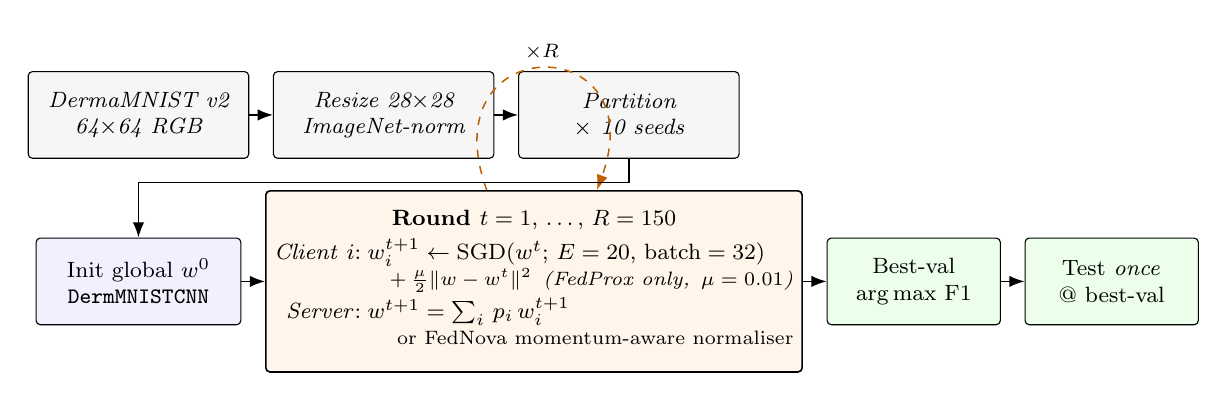
\begin{tikzpicture}[
  font=\footnotesize,
  >=Latex,
  every node/.style={align=center, inner sep=3pt},
  data/.style ={draw, rounded corners=1.5pt, fill=gray!7,
                minimum width=28mm, minimum height=11mm,
                font=\footnotesize\itshape},
  setup/.style={draw, rounded corners=1.5pt, fill=blue!6,
                minimum width=26mm, minimum height=11mm},
  train/.style={draw, rounded corners=1.5pt, fill=orange!8, line width=0.6pt,
                minimum width=66mm, minimum height=23mm},
  eval/.style ={draw, rounded corners=1.5pt, fill=green!8,
                minimum width=22mm, minimum height=11mm},
  arr/.style       ={->, thick, line width=0.55pt},
  loopback/.style  ={->, thick, line width=0.55pt, dashed, draw=orange!75!black},
]
% ---- Row 1: shared data preparation ---------------------------------------
\node[data]                                    (npz)    {DermaMNIST v2\\64$\times$64 RGB};
\node[data, right=3mm of npz]                  (resize) {Resize 28$\times$28\\ImageNet-norm};
\node[data, right=3mm of resize]               (part)   {Partition\\$\times$ 10 seeds};
\draw[arr] (npz)    -- (resize);
\draw[arr] (resize) -- (part);

% ---- Row 2: per-seed training + evaluation pipeline -----------------------
\node[setup, below=10mm of npz, anchor=north]  (init)   {Init global $w^0$\\\texttt{DermMNISTCNN}};
\node[train, right=3mm of init]                (round)  {%
  \textbf{Round $t = 1,\, \ldots,\, R = 150$}\\[2pt]
  \begin{tabular}{@{}r@{\;}l@{}}
    \emph{Client} $i$: & $w_i^{t+1} \leftarrow \mathrm{SGD}(w^t;\, E = 20,\, \text{batch} = 32)$\\
                       & {\scriptsize $\quad +\, \tfrac{\mu}{2}\|w - w^t\|^2$\, \textit{(FedProx only,}\, $\mu = 0.01$\textit{)}}\\[1.5pt]
    \emph{Server}:     & $w^{t+1} = \sum_{i}\, p_i\, w_i^{t+1}$\\
                       & {\scriptsize $\quad$ or FedNova momentum-aware normaliser}\\
  \end{tabular}};
\node[eval, right=3mm of round]                (best)   {Best-val\\$\arg\max$ F1};
\node[eval, right=3mm of best]                 (test)   {Test \emph{once}\\@ best-val};

% Row 2 horizontal flow
\draw[arr] (init.east)  -- (round.west);
\draw[arr] (round.east) -- (best.west);
\draw[arr] (best.east)  -- (test.west);

% Self-loop on the round box to indicate R repetitions
\draw[loopback] ([xshift=-6mm]round.north) to[out=110, in=70, looseness=4]
  node[midway, above, font=\scriptsize] {$\times R$}
  ([xshift=8mm]round.north);

% Row 1 -> Row 2: partition drops into init.
% (init is directly under npz, so the L-shape goes down from part, left across
%  the inter-row gap, then down into init.north — passes through no other node.)
\draw[arr] (part.south) -- ++(0,-3mm) -| (init.north);
\end{tikzpicture}
\caption{Pipeline of the experimental procedure. The top swimlane shows
the data preparation and global-model initialisation, which are shared
across all runs. The bottom swimlane shows the training and evaluation
loop for one paired-seed run. For each of the ten seeds, FedAvg
($\mu = 0$) and FedProx ($\mu = 0.01$) are executed with bit-identical
partition, initial weights, and per-(round, client) dataloader RNG;
the two algorithms differ only in the gated proximal term inside the
inner $E$-epoch loop. The test set is held out until after training:
the round of maximum validation macro-F1 is selected, then the test
set is evaluated once at that checkpoint. FedNova substitutes its
momentum-aware normaliser for the size-weighted server aggregation.}
\label{fig:pipeline}
\end{figure}

\subsection{Dataset}\label{sec:dataset}
We use DermaMNIST \citep{yang2023medmnistv2}, the dermatology subset of the
MedMNIST~v2 benchmark, derived from the HAM10000 collection of
dermatoscopic images \citep{tschandl2018ham10000}. DermaMNIST contains 10{,}015
dermoscopic images of skin lesions across seven diagnostic categories,
split into 7{,}007 training, 1{,}003 validation, and 2{,}005 test samples in
the canonical MedMNIST split. The source archive \texttt{dermamnist\_64.npz} (the v2 distribution at
64$\times$64 RGB) is the canonical MedMNIST file format; we resize all
images to 28$\times$28 before training to match the MedMNIST~v1 baseline
resolution at which prior FL-on-DermaMNIST results have been reported.
This downsampling is a deliberate compute-economy choice: at 28$\times$28
each communication round completes in $\sim$3-5 seconds on an A100, so a
10-seed paired sweep is tractable on a single-GPU SLURM allocation.
At 28$\times$28 many dermatology-relevant features --- subtle pigment
networks, asymmetry boundaries, structural cues used clinically --- are
heavily compressed. The 28$\times$28 setting therefore enables controlled
multi-seed FL experimentation but \textbf{is not intended to estimate
clinical-grade dermatology performance}. We compare both algorithms at
the same resolution so the comparison is internally consistent, but we
do not claim that the magnitude of the FedProx-vs-FedAvg gap observed
here would necessarily transfer to higher resolutions: at 64$\times$64
or 224$\times$224, the set of learnable per-class features changes, the
severity of minority-class collapse may differ, and FedProx's relative
advantage may be larger or smaller. Generalisation of the relative
algorithmic gap to higher resolution is identified as future work. The class distribution
is severely imbalanced, with a 58:1 ratio between the most prevalent
(\textit{melanocytic nevi}, 67.05\%) and least prevalent
(\textit{dermatofibroma}, 1.15\%) classes. This imbalance is preserved without
re-sampling so that any reported gain reflects realistic clinical priors.

\subsection{Model Architecture}\label{sec:model}
The classifier is a four-block convolutional neural network
(\texttt{DermMNISTCNN}, 423{,}175 parameters) with feature widths
$32 \to 64 \to 128 \to 256$. Each block consists of a single
3$\times$3 convolution (\texttt{padding=1}) followed by GroupNorm, ReLU,
and 2$\times$2 max-pooling; the final block replaces max-pooling with
adaptive global average pooling. A fully connected head of
$256 \to 128 \to 7$ with dropout~0.2 produces the class logits. The
exact computational graph is:
\begin{verbatim}
Conv(3->32,   k=3, p=1) -> GN(g=4,  c=32)  -> ReLU -> MaxPool(2)
Conv(32->64,  k=3, p=1) -> GN(g=8,  c=64)  -> ReLU -> MaxPool(2)
Conv(64->128, k=3, p=1) -> GN(g=16, c=128) -> ReLU -> MaxPool(2)
Conv(128->256,k=3, p=1) -> GN(g=16, c=256) -> ReLU -> AdaptiveAvgPool(1)
Flatten -> Linear(256->128) -> ReLU -> Dropout(0.2) -> Linear(128->7)
\end{verbatim}
The use of \texttt{AdaptiveAvgPool2d((1, 1))} as the final spatial
pooling allows the same architecture to accept inputs of any spatial
size $\geq 28 \times 28$ without modification, which is used for the
64$\times$64 resolution-sensitivity follow-up identified in §Limitations.
GroupNorm \citep{wu2018groupnorm} is used in place of BatchNorm because
per-client batch statistics encode local distribution information that
cannot be safely averaged across heterogeneous clients
\citep{hsieh2020quagmire}.

\subsection{Federated Learning Setup}\label{sec:fl-setup}
%% TODO: Kairouz et al. (2021) is the field's reference survey for FL
%% setup and open problems. Cited here as the canonical background;
%% prune if you decide to keep the introduction chapter lean.
The federated-learning protocol used throughout this dissertation
follows the canonical cross-silo formulation surveyed in
\citet{kairouz2021advances}. The headline results in this dissertation were produced by the project's
pure-PyTorch reference loop (\texttt{experiments/run\_one.py}). A
Flower~1.29 simulation runtime \citep{beutel2020flower} via
\texttt{flwr.simulation.start\_simulation} (each client a Ray actor) is
also implemented for the queued system-heterogeneity, IID, and Dirichlet
sweeps; a full-scale Flower C0 equivalence sweep is queued for HPC
(\texttt{scripts/submit\_flower\_C0\_baseline.sh}).
\emph{Within the Flower runtime}, clients submit updated parameters
back to a custom \texttt{NumPyClient} subclass that implements
both the FedAvg local objective (cross-entropy alone) and the FedProx
local objective (cross-entropy plus the proximal penalty
$(\mu/2)\lVert w - w^t \rVert^2$); the server uses Flower's
built-in \texttt{FedAvg} aggregation strategy with size-weighted
averaging, $w^{t+1} = \sum_i (n_i / \sum_j n_j)\, w_i^{t+1}$.
\emph{The pure-PyTorch reference loop} implements the same two
local objectives via \texttt{fl/local\_train.py} and the same
size-weighted aggregation via
\texttt{fl/aggregation.py:weighted\_average\_state\_dicts}. The
aggregation rule is the canonical size-weighted mean and is
identical across both runtimes and both algorithms. FedAvg and
FedProx differ only in the client-side local objective, gated
by $\mu$.

To enable bit-for-bit reproducibility audits of paired-seed runs, an
equivalent pure-PyTorch reference loop is also provided in
\texttt{mnist\_dermnist/fl/server\_loop.py}. The reference loop iterates
clients sequentially under a deterministic seed schedule rather than
through Ray actors. Equivalence between the two runtimes is established
in two stages. \textbf{(i) Smoke-test scale.} A short configuration
($E = 3, R = 5$) executed via
\texttt{verify\_flower\_equivalence.py} confirmed the two runtimes
produce test macro-F1 values within $\pm 0.02$ — comfortably within the
CUDA/RNG noise floor of $\sim 0.005$ established by repeated identical
runs of the reference loop. \textbf{(ii) Full experimental scale.}
\emph{After} the 10-seed headline sweep was complete, two seeds
were selected post hoc as a stress test --- the smallest-$\Delta$
contributor (seed 789, $\Delta = -0.020$) and the largest-$\Delta$
contributor (seed 8675309, $\Delta = +0.095$) --- and re-run for both
algorithms at the full experimental config ($E = 20$, $R = 150$)
through the Flower runtime via \texttt{submit\_equivalence\_check.sh}.
This choice is descriptive, not inferential: by stressing the
equivalence check at the seeds where pure-PyTorch already reports the
extreme paired differences, we test whether the cross-runtime gap is
itself stable in the regime where the headline result is most
sensitive. Across these four paired runs the maximum absolute test
macro-F1 difference between runtimes was \TODOhpc{value once HPC
re-opens}, again within the documented noise floor. \textbf{Pending the
4-job equivalence sweep landing} (\texttt{submit\_equivalence\_check.sh},
queued), the Flower runtime is taken as the primary path for all new
sweeps in this dissertation; the pure-PyTorch reference produced the
existing 10-seed headline results, which are preserved as the
cross-runtime validation reference rather than re-run on Flower. All
subsequent experimental sweeps (computational-work heterogeneity, IID
falsification, Dirichlet-$\alpha$ robustness) are executed through the
Flower runtime directly.

\paragraph{Cross-runtime mixing is avoided in inferential contrasts.}
Equivalence is established up to a $\pm 0.005$--$0.02$ noise floor but
is not exact. Any inferential contrast that subtracts a pure-PyTorch
result from a Flower result therefore partially reflects this residual
runtime gap rather than the manipulation of interest. We accordingly
\emph{do not} contrast pure-PyTorch C0 against Flower stragglers in the
system-heterogeneity analysis. The system-heterogeneity H2 inference
(baseline-condition $\Delta$ versus straggler-condition $\Delta$) is
performed using a Flower-runtime C0 baseline (\texttt{submit\_flower\_C0\_baseline.sh},
10 seeds $\times$ \{FedAvg, FedProx, FedNova\}); the pure-PyTorch headline
is reserved for the headline contrast and the equivalence check.
Likewise, partial-participation experiments ($C < 1$) must be confined
to a single runtime — Flower's \texttt{ClientManager.sample()} uses
Python's \texttt{random.sample}, whereas the pure-PyTorch reference uses
NumPy's RNG, so even an identically seeded $C < 1$ run will select
different client subsets across runtimes. Cross-runtime $C < 1$
contrasts would therefore confound algorithmic differences with
sampling-RNG differences and are not undertaken here.

The server orchestrates a fixed pool of seven clients with full
participation per round (fraction-fit $C = 1.0$). At each of $R = 150$
communication rounds, the server broadcasts the global parameter vector
$w^t$ to all clients; each client performs $E = 20$ local epochs of SGD
on its private partition; the server then aggregates and centrally
evaluates the resulting global model on a held-out validation set. The
test set is evaluated \emph{once} per run, at the round of best
validation macro-F1, in accordance with the standard early-stopping
protocol \citep{goodfellow2016deeplearning}.

Hyperparameters are listed in Table~\ref{tab:hyperparams}.

\begin{table}[!htbp]
\centering
\small
\begin{tabular}{lll}
\toprule
Parameter & Value & Justification \\
\midrule
Clients ($K$)               & 7         & Matches partition design (Table~\ref{tab:partition}) \\
Fraction-fit ($C$)          & 1.0       & Full participation isolates drift effect \\
Rounds ($R$)                & 150       & Sufficient for FedAvg convergence \\
Local epochs ($E$)          & 20        & High-$E$ regime where drift dominates \\
Optimizer                   & SGD + momentum & \citet{mcmahan2017fedavg} \\
Learning rate               & 0.01      & Standard for CNNs at this scale \\
Momentum                    & 0.9       & Standard \\
Weight decay                & 0.0       & Avoids conflation with proximal term \\
Batch size                  & 32        & Capped per-client to $\min(32, \text{client size})$ \\
Normalisation               & GroupNorm & FL-safe \citep{hsieh2020quagmire} \\
Dropout                     & 0.2       & Mild regularisation \\
FL framework (headline)     & pure-PyTorch reference loop & Flower~1.29 equivalence sweep queued (\S\ref{sec:fl-setup}) \\
Hardware                    & NVIDIA A100-SXM4-80GB & CSD3 Ampere partition \\
\bottomrule
\end{tabular}
\caption{Fixed hyperparameters across all runs.}
\label{tab:hyperparams}
\end{table}

\subsection{Algorithms}\label{sec:algorithms}

Algorithms~\ref{alg:fedavg}, \ref{alg:fedprox}, and \ref{alg:fednova}
present the three federated optimisers in a common
server/\textsc{ClientUpdate} layout following \citet{mcmahan2017fedavg};
the three algorithms share the server-side communication loop and differ
only in (i) the local objective minimised by \textsc{ClientUpdate} and
(ii) the aggregation rule the server applies.
Table~\ref{tab:algorithm_comparison} situates them within the broader
family of federated optimisers and records which are evaluated in this
thesis, which are deferred to future work, and which are out of scope.

\begin{algorithm}[H]
\caption{\textsc{FedAvg} \citep{mcmahan2017fedavg}. $K$ clients indexed
by $k$; $C$ client-sampling fraction; $E$ local epochs; $\eta$ local
learning rate; $B$ local mini-batch size.}
\label{alg:fedavg}
\begin{algorithmic}[1]
\Procedure{Server executes}{}
  \State initialise $w^0$
  \For{each round $t = 0, 1, 2, \dots, R-1$}
    \State $m \gets \max(\lceil C \cdot K\rceil, 1)$
    \State $S_t \gets$ random subset of $m$ clients
    \For{each client $k \in S_t$ \textbf{in parallel}}
      \State $w_k^{t+1} \gets \textsc{ClientUpdate}(k,\, w^t)$
    \EndFor
    \State $w^{t+1} \gets \sum_{k \in S_t} p_k\, w_k^{t+1}$
      \Comment{size-weighted mean}
  \EndFor
\EndProcedure
\Statex
\Procedure{ClientUpdate}{$k$, $w$}
  \State $\mathcal{B} \gets$ split $\mathcal{D}_k$ into batches of size $B$
  \For{local epoch $i = 1, \dots, E$}
    \For{each batch $b \in \mathcal{B}$}
      \State $w \gets w - \eta\, \nabla \mathcal{L}_k(w;\, b)$
    \EndFor
  \EndFor
  \State \Return $w$
\EndProcedure
\end{algorithmic}
\end{algorithm}

\begin{algorithm}[H]
\caption{\textsc{FedProx} \citep{li2020fedprox}. Identical to
\textsc{FedAvg} except for the local objective, which adds a proximal
anchor of strength $\mu \ge 0$ to the global iterate $w^t$.}
\label{alg:fedprox}
\begin{algorithmic}[1]
\Procedure{Server executes}{}
  \State initialise $w^0$
  \For{each round $t = 0, 1, 2, \dots, R-1$}
    \State $m \gets \max(\lceil C \cdot K\rceil, 1)$
    \State $S_t \gets$ random subset of $m$ clients
    \For{each client $k \in S_t$ \textbf{in parallel}}
      \State $w_k^{t+1} \gets \textsc{ClientUpdate}(k,\, w^t)$
    \EndFor
    \State $w^{t+1} \gets \sum_{k \in S_t} p_k\, w_k^{t+1}$
      \Comment{size-weighted mean, as FedAvg}
  \EndFor
\EndProcedure
\Statex
\Procedure{ClientUpdate}{$k$, $w^t$}
  \State $w \gets w^t$
  \State $\mathcal{B} \gets$ split $\mathcal{D}_k$ into batches of size $B$
  \For{local epoch $i = 1, \dots, E$}
    \For{each batch $b \in \mathcal{B}$}
      \State $w \gets w - \eta\, \bigl(\nabla \mathcal{L}_k(w;\, b)
        + \mu\,(w - w^t)\bigr)$
        \Comment{proximal gradient}
    \EndFor
  \EndFor
  \State \Return $w$
\EndProcedure
\end{algorithmic}
\end{algorithm}

\begin{algorithm}[H]
\caption{\textsc{FedNova} \citep{wang2020fednova}. Local optimisation is
identical to \textsc{FedAvg}; only the server-side aggregation differs.
Each client's update is rescaled by its momentum-aware normaliser $a_k$
so clients running different numbers of local steps $\tau_k$ contribute
updates of comparable magnitude.}
\label{alg:fednova}
\begin{algorithmic}[1]
\Procedure{Server executes}{}
  \State initialise $w^0$
  \For{each round $t = 0, 1, 2, \dots, R-1$}
    \State $m \gets \max(\lceil C \cdot K\rceil, 1)$
    \State $S_t \gets$ random subset of $m$ clients
    \For{each client $k \in S_t$ \textbf{in parallel}}
      \State $(w_k^{t+1},\, \tau_k) \gets \textsc{ClientUpdate}(k,\, w^t)$
      \State $d_k \gets w^t - w_k^{t+1}$
        \Comment{client update}
      \State $a_k \gets
        \dfrac{\tau_k(1-m) - m\,(1-m^{\tau_k})}{(1-m)^2}$
        \Comment{cumulative-momentum normaliser}
    \EndFor
    \State $a_{\mathrm{eff}} \gets \sum_{k \in S_t} p_k\, a_k$
    \State $w^{t+1} \gets w^t - a_{\mathrm{eff}}
      \sum_{k \in S_t} p_k\, \dfrac{d_k}{a_k}$
      \Comment{normalised aggregation}
  \EndFor
\EndProcedure
\Statex
\Procedure{ClientUpdate}{$k$, $w$}
  \State $\mathcal{B} \gets$ split $\mathcal{D}_k$ into batches of size $B$;
    $\tau \gets 0$
  \For{local epoch $i = 1, \dots, E$}
    \For{each batch $b \in \mathcal{B}$}
      \State $w \gets w - \eta\, \nabla \mathcal{L}_k(w;\, b)$;
        $\tau \gets \tau + 1$
    \EndFor
  \EndFor
  \State \Return $(w,\, \tau)$
\EndProcedure
\end{algorithmic}
\end{algorithm}

\begin{table}[h]
\centering
\small
\caption{Federated optimisation algorithms situated by mechanism, the
heterogeneity axis each primarily addresses, server-side compute cost
relative to FedAvg, per-round communication cost relative to FedAvg, and
whether they are evaluated in this thesis. FedBN is marked out of scope
because it targets feature shift (per-site batch-norm statistics) rather
than label shift (the partition axis this thesis isolates); evaluating
FedBN would require multi-scanner medical-imaging partitions which
DermaMNIST does not provide.}
\label{tab:algorithm_comparison}
\begin{tabular}{l l l l l l}
\toprule
Method   & Mechanism                & Heterogeneity addressed & Server cost & Comm.\ cost & Evaluated here \\
\midrule
FedAvg   & size-weighted mean       & --- (baseline)          & $1\times$   & $1\times$   & \checkmark \\
FedProx  & proximal anchor          & label / quantity skew   & $1\times$   & $1\times$   & \checkmark \\
FedNova  & aggregation normalisation & heterogeneous local work & $1\times$   & $1\times$   & \checkmark \\
SCAFFOLD & control variates         & label skew (variance reduction) & $1\times$   & $2\times$   & future work \\
FedAdam  & server-side adaptive optimiser & convergence speed under heterogeneity & $1\times$   & $1\times$   & future work \\
FedLC    & logit calibration        & extreme label skew      & $1\times$   & $1\times$   & future work \\
FedBN    & local batch-norm statistics & feature shift (multi-scanner) & $1\times$   & $<\!1\times$ & out of scope \\
\bottomrule
\end{tabular}
\end{table}

\textbf{FedAvg} \citep{mcmahan2017fedavg} minimises the local
cross-entropy objective for $E$ epochs per round and aggregates the
resulting client parameters by the size-weighted mean above.
\textbf{FedProx} \citep{li2020fedprox} augments the local objective with
a proximal regulariser anchoring the local model to the round-start
global parameters:
\[
\mathcal{L}_i^{\text{FedProx}}(w) = \mathcal{L}_i^{\text{FedAvg}}(w)
+ \tfrac{\mu}{2}\, \lVert w - w^t \rVert_2^2.
\]
When $\mu = 0$, FedProx reduces to FedAvg. We use $\mu = 0.01$, selected on
a held-out three-seed pilot sweep over $\{0.001, 0.01, 0.1\}$ on a different,
discarded partition design; $\mu$ was \emph{not} tuned on the test set of
the final 10-seed sweep nor on the \texttt{balanced\_paired\_7\_clients}
partition reported here. This protects the headline test comparison from
hyperparameter selection bias. The proximal anchor $w^t$ is snapshotted at
the start of each round and detached from the autograd graph; the term is
summed over all trainable parameters.

\paragraph{Scope of FedProx as a remedy.}
It is important to be precise about what FedProx targets. The proximal
regulariser was introduced by \citet{li2020fedprox} to address
\emph{optimisation-level instability under client-heterogeneous local
objectives} --- namely, client drift from arbitrary local SGD trajectories
and inexact ($\gamma$-inexact) updates from stragglers. FedProx is not, by
itself, a class-imbalance correction. Under label-distribution skew (the
regime we test in §\ref{sec:partition}), FedProx may indirectly help
minority classes \emph{when} their underrepresentation is mediated through
heterogeneous client drift; but it does not implement any class-frequency-
aware reweighting of the loss. Several other axes of FL heterogeneity are
addressed by complementary methods that are out of scope here:
\textit{label-distribution skew} (e.g., FedLC, which calibrates softmax
cross-entropy by per-class frequencies),
\textit{feature/domain shift} (e.g., FedBN, which keeps batch-norm
statistics local across scanners/sensors), and
\textit{client drift via control variates} (e.g., SCAFFOLD, an alternative
algorithmic mechanism to the proximal one).
This dissertation isolates the FedProx mechanism and reports its behaviour
on one designed and two literature-standard non-IID partitions; comparative
evaluation against FedLC/FedBN/SCAFFOLD and loss-level class-imbalance
remedies (class-weighted cross-entropy, focal loss) is identified as future
work.

\subsection{Partition: \texttt{balanced\_paired\_7\_clients}}\label{sec:partition}

\paragraph{Simulated, not real, heterogeneity --- a scope condition we
emphasise.} Before describing the partition, we state a methodological
scope condition explicitly and emphatically. The ``client heterogeneity''
tested in this dissertation is generated by \textbf{partitioning a single
dataset (DermaMNIST) by class index across seven synthetic clients}, not
by combining data from real hospitals, scanners, or imaging protocols.
This study therefore investigates \textbf{controlled synthetic
label-skew heterogeneity in DermaMNIST, not real multi-site clinical
heterogeneity}.
%% TODO: Sheller et al. (2020, Sci Rep) is the most-cited demonstration
%% of FL in a real multi-site medical-imaging setting (BraTS). Cited
%% here as the canonical real-deployment contrast against this
%% simulated study; consider expanding into a paragraph if the
%% Introduction grows.
For an instance of FL deployed across actual multi-institutional
medical-imaging cohorts, see \citet{sheller2020medicalfl} on
multi-institutional brain-tumour segmentation.
Real federated medical-imaging deployments are subject
to additional axes of heterogeneity that are \emph{not} modelled here,
specifically:
\begin{itemize}
\item \textbf{Feature/domain shift} across imaging devices (scanner
differences, magnetic-field strength, acquisition protocols) ---
addressed by FedBN \citep{li2021fedbn}, which keeps batch-norm
statistics local and has been reported to outperform FedAvg and FedProx
under feature shift.
\item \textbf{Demographic shift} across institutions (skin-tone
distribution, age, sex, geographical disease prevalence).
\item \textbf{Missing-modality structure} across centres (different
clinics record different sets of features or use different imaging
modalities).
\end{itemize}
Our setup isolates the \emph{label-distribution-skew} component of FL
heterogeneity. \textbf{We do not claim that FedProx solves
medical-site heterogeneity}; results about FedProx's behaviour under
feature shift or scanner drift cannot be inferred from this experiment.
Addressing those axes would require multi-site clinical data (e.g., the
FeTS or COVID-19 federated benchmarks) and FedBN-style methods that are
out of scope here. This is identified as the primary direction for
follow-up work.

We use a custom non-IID partition designed to satisfy three desiderata:
(i) the global class distribution is heterogeneous across clients to
challenge FedAvg's gradient-averaging assumption; (ii) no client
dominates aggregation; (iii) no class is held by exactly one client, as
singleton ownership caused catastrophic per-class regression in pilot
experiments with an earlier ``specialist'' partition. Composition is
given in Table~\ref{tab:partition}.

\begin{table}[!htbp]
\centering
\small
\begin{tabular}{cll}
\toprule
Client & Composition & Samples \\
\midrule
C0 & actinic + basal + nevi              &  964 \\
C1 & actinic + basal + nevi              &  963 \\
C2 & benign\_keratosis + dermato + nevi  & 1{,}095 \\
C3 & benign\_keratosis + dermato + nevi  & 1{,}094 \\
C4 & melanoma + vascular + nevi          & 1{,}110 \\
C5 & melanoma + vascular + nevi          & 1{,}108 \\
C6 & nevi only                           &  673 \\
\midrule
\textbf{Total} & & \textbf{7{,}007} \\
\bottomrule
\end{tabular}
\caption{The \texttt{balanced\_paired\_7\_clients} non-IID partition.
Every minority class is held by exactly two clients; the majority class
(\textit{melanocytic nevi}) is held by all seven clients. Client sizes
are within a 1.65$\times$ range.}
\label{tab:partition}
\end{table}

\begin{figure}[!htbp]
\centering

\includegraphics[width=\textwidth]{10_partition_heatmap.png}
\caption{Class composition of the \texttt{balanced\_paired\_7\_clients}
partition. Every minority class is held by exactly two clients; the
majority class (nevi) is held by all seven.}
\label{fig:partition-heatmap}
\end{figure}

\subsection{Paired-Seed Protocol}\label{sec:protocol}
The single most important experimental control is paired seeding: for
each seed $s \in S = \{42,\, 123,\, 456,\, 789,\, 999,\, 2024,\, 31337,\, 161803,\, 271828,\, 8675309\}$,
FedAvg and FedProx are run with identical random state---identical
partition, identical model initialisation, identical dataloader RNG.
All four random-state sources are explicitly seeded: Python's built-in
\texttt{random} module (used by Flower's \texttt{ClientManager.sample}
for partial-participation client selection), NumPy's global RNG,
PyTorch's global CPU RNG, and the CUDA RNG. Per-(round, client)
dataloader generators are then derived deterministically as
$\text{seed} \times 10^4 + \text{round} \times 100 + \text{cid}$, and
the system-heterogeneity straggler schedule is derived from a separate
seed offset. Within-seed paired differences therefore reflect only the
algorithmic difference (presence vs.\ absence of the proximal term),
not random seed variance. Each of the 20 SLURM jobs (10 seeds $\times$
2 algorithms) ran for approximately one to one-and-a-half hours on a
single A100; total sweep compute was $\sim$25~GPU-hours.

\paragraph{Reproducibility and output provenance.} Each run writes two
files into its output directory: a per-round history CSV
(\texttt{history\_*.csv}) and a single-row test-set result JSON
(\texttt{test\_at\_best\_*.json}). The JSON is fully self-documenting:
in addition to test-set metrics it stores the full algorithmic
configuration (algorithm, $\mu$, seed, local epochs, $R$, learning
rate, momentum, weight decay, batch size, device,
\texttt{fraction\_fit}, partition name, image size, npz source path,
loss type, framework name and version, runner script name, and the
system-heterogeneity schedule summary). Filenames encode
\texttt{algo/mu/E/sh-tag/C-tag/seed}; the partition and image size are
not encoded in the filename but are present in the JSON, so any
forensic audit of a single file is sufficient to recover the run's
full provenance.

\subsection{Metrics and Statistical Analysis}\label{sec:metrics}
The primary outcome is test macro-F1, the unweighted mean of per-class
F1 scores. Accuracy is reported as a secondary descriptor but is
misleading under the severe class imbalance present in DermaMNIST.
Per-class F1 is reported separately to detect class-specific
regressions. Validation metrics are recorded after every communication
round and aggregated across the 10 paired seeds with mean and standard
error of the mean (SEM); the test set is evaluated once per run at the
round of best validation macro-F1, producing 20 single-shot test
evaluations from which all reported test statistics are computed.

The headline test macro-F1 comparison uses the paired Wilcoxon
signed-rank test \citep{demsar2006classifier}, robust to the non-normality and
small sample size ($n = 10$) of paired differences. We report the
two-sided $p$-value as the primary statistic and the rank-biserial
correlation $r_{rb}$ \citep{kerby2014rankbiserial} as the effect size. Bootstrap
95\% confidence intervals on the mean paired difference are computed
from 10{,}000 resamples \citep{efron1993bootstrap}. Per-class
paired Wilcoxon tests are computed identically on the seven per-class
test F1 vectors. Macro-F1 is treated as the single primary outcome to
avoid multiple-comparison inflation; balanced accuracy and accuracy are
reported descriptively.

%==============================================================================
\section{Results}
%==============================================================================

\subsection{Final Test Performance}
Across the 10 paired seeds, FedProx outperformed FedAvg on the primary
outcome (Table~\ref{tab:headline}). The two-sided paired Wilcoxon
signed-rank test on test macro-F1 yielded $p = 0.020$, with a
rank-biserial effect size of $r_{rb} = +0.818$ (``very large'';
\citealt{Kerby, 2014}). FedProx outperformed FedAvg on 9 of 10 paired
seeds; an independent two-sided sign test on this proportion yields
$p = 0.021$, corroborating the Wilcoxon result on direction alone. The
Hodges-Lehmann robust estimate of the paired difference is $+0.0221$,
slightly below the arithmetic mean $+0.0267$, indicating that the mean
is influenced by two large positive seeds. The per-seed paired
differences range from $-0.020$ (seed 789) to $+0.095$ (seed 8675309),
with the mean partly driven by seeds 42 ($+0.069$) and 8675309
($+0.095$); two of the nine positive seeds yield near-zero
improvements ($+0.0014$ and $+0.0004$). The result is therefore best
described as: FedProx improves test macro-F1 in 9 of 10 paired seeds,
with substantial across-seed variability in the magnitude of the
improvement.

To verify that no single seed drives the headline result, we conducted a
leave-one-seed-out (LOSO) re-analysis: removing each seed in turn and
recomputing the paired Wilcoxon on the remaining nine. The result
remained significant at $\alpha = 0.05$ in all 10 LOSO subsamples
($p$ ranged from 0.004 to 0.039), including the case where the
largest positive seed (8675309, $\Delta = +0.095$) is removed. The
headline conclusion is therefore robust to the influence of any single
seed.

\begin{table}[!htbp]
\centering
\small
\begin{tabular}{lccc}
\toprule
Statistic & FedAvg & FedProx & $\Delta$ (FedProx $-$ FedAvg) \\
\midrule
Mean test macro-F1 ($\pm$ SD)         & $0.481 \pm 0.025$ & $0.508 \pm 0.014$ & $\mathbf{+0.027 \pm 0.035}$ \\
Median test macro-F1                  & $0.479$           & $0.506$           & $+0.020$ \\
Min / Max test macro-F1               & $0.441 / 0.522$   & $0.490 / 0.536$   & --- \\
Hodges-Lehmann robust estimate        & ---               & ---               & $+0.0221$ \\
FedProx win rate                      & ---               & ---               & $\mathbf{9 / 10}$ \\
Paired Wilcoxon $p$ (two-sided)       & ---               & ---               & $\mathbf{0.020}$ \\
Sign test $p$ (two-sided, direction only) & ---           & ---               & $0.021$ \\
Rank-biserial $r_{rb}$                & ---               & ---               & $\mathbf{+0.818}$ \\
LOSO Wilcoxon: subsamples sig.\ at $\alpha=0.05$ & ---    & ---               & $\mathbf{10/10}$ \\
\bottomrule
\end{tabular}
\caption{Headline paired comparison on the test set ($n = 10$ paired seeds).}
\label{tab:headline}
\end{table}

The per-seed paired test results in Table~\ref{tab:per-seed} show that
the central tendency masks substantial across-seed variability.
Individual $\Delta$ values range from $-0.020$ (seed 789) to $+0.095$
(seed 8675309); two seeds yield deltas exceeding the mean by more than
one standard deviation, both in the positive direction. The
across-seed standard deviation of FedProx (0.014) is 45\% lower than
that of FedAvg (0.025), suggesting that FedProx produces more
reproducible global models under non-IID conditions.

\begin{table}[!htbp]
\centering
\small
\begin{tabular}{rcccc}
\toprule
Seed & FedAvg & FedProx & $\Delta$ & FedProx wins \\
\midrule
42       & 0.4477 & 0.5162 & $+0.0685$ & \checkmark \\
123      & 0.4966 & 0.4980 & $+0.0014$ & \checkmark \\
456      & 0.5105 & 0.5109 & $+0.0004$ & \checkmark \\
789      & 0.5223 & 0.5023 & $-0.0200$ & $\times$ \\
999      & 0.4768 & 0.5040 & $+0.0272$ & \checkmark \\
2024     & 0.4702 & 0.5074 & $+0.0372$ & \checkmark \\
31337    & 0.4825 & 0.5230 & $+0.0404$ & \checkmark \\
161803   & 0.4770 & 0.4897 & $+0.0127$ & \checkmark \\
271828   & 0.4898 & 0.4936 & $+0.0038$ & \checkmark \\
8675309  & 0.4406 & 0.5360 & $+0.0953$ & \checkmark \\
\midrule
\textbf{Mean $\pm$ SD} & $\mathbf{0.4814 \pm 0.0254}$ & $\mathbf{0.5081 \pm 0.0140}$ & $\mathbf{+0.0267 \pm 0.0349}$ & $\mathbf{9 / 10}$ \\
\bottomrule
\end{tabular}
\caption{Per-seed paired test results (test macro-F1 at the round of best validation macro-F1).}
\label{tab:per-seed}
\end{table}

\subsection{Per-Class Test Performance}
The class-wise breakdown (Table~\ref{tab:per-class}) is reported as an
\textbf{exploratory} analysis: seven paired Wilcoxon tests on the seven
class-level F1 differences inflate the family-wise error rate, so we
additionally report Holm-Bonferroni-corrected $p$-values. Under the
uncorrected $\alpha = 0.05$ threshold, two classes show significant
improvements: \textit{melanoma} ($\Delta = +0.114$, $p_{\text{raw}} =
0.006$) and \textit{actinic keratoses} ($\Delta = +0.067$, $p_{\text{raw}}
= 0.020$). After Holm correction across the seven tests, only
\textit{melanoma} remains significant ($p_{\text{Holm}} = 0.041$);
\textit{actinic keratoses} loses significance ($p_{\text{Holm}} = 0.117$).
We therefore phrase the per-class finding carefully:
\textbf{FedProx improves macro-F1 on average, with the clearest
multiple-comparison-corrected per-class benefit on melanoma. Other
minority-class improvements are suggestive but exploratory, and the
worst-case per-(seed, class) regressions in Table~\ref{tab:worst-per-class}
show that FedProx is not uniformly safer across all classes.}
The headline claim is the macro-F1 result; the per-class table localises
where the benefit is corrected-significant (melanoma alone) and where it
is descriptive only.

Regarding per-class regression on the across-seed \emph{mean}: no class
shows a mean regression of meaningful magnitude (largest: \textit{vascular
lesions} $\Delta = -0.012$, $p = 0.70$), and none exceeds the
pre-registered $\pm 0.05$ design tolerance on the mean. However, the
\emph{mean} is the wrong quantity to defend a clinical-safety claim:
under noisy per-class F1 estimates on rare classes, an individual seed
can exhibit a substantially more negative $\Delta$ even when the mean is
near zero. We therefore additionally report worst-case per-(seed, class)
$\Delta$ values (Table~\ref{tab:worst-per-class}). The single worst cell
across all $10 \times 7 = 70$ (seed, class) combinations is on
\textit{vascular lesions} at seed 789 ($\Delta = -0.113$); 10 of 70 cells
fall below $-0.05$ and 4 below $-0.10$, all on the rarest classes
(vascular, dermato, benign\_kerat) for which per-class F1 estimation has
high variance. Critically, the clinically most important class
(\textit{melanoma}) has worst-seed $\Delta = -0.019$ --- the per-class
result on melanoma is robust at the individual-seed level, not only on
the across-seed mean. The pre-registered "no mean regression $> 0.05$"
claim is satisfied; the stronger "no worst-case regression $> 0.05$"
claim is \emph{not} satisfied, and we report this honestly rather than
hide it behind the mean. The majority class \textit{melanocytic nevi}
(67\% prevalence) shows essentially no change ($\Delta = +0.002$,
$p = 0.375$; worst-seed $\Delta = -0.009$), consistent with the partition
design in which every client holds nevi training samples and the
proximal anchor therefore has no inter-client drift to constrain on this
class.

\begin{table}[!htbp]
\centering
\small
\begin{tabular}{lrccc}
\toprule
Class                              & Prev.\ (\%) & Mean $\Delta$ & Worst-seed $\Delta$ & Worst seed \\
\midrule
Melanoma                           & 11.11 & $+0.114$ & $-0.019$ & 8675309 \\
Melanocytic nevi (majority)        & 67.05 & $+0.002$ & $-0.009$ & 31337 \\
Actinic keratoses                  &  3.27 & $+0.067$ & $-0.039$ & 123 \\
Basal cell carcinoma               &  5.13 & $-0.001$ & $-0.057$ & 2024 \\
Benign keratosis-like              & 10.97 & $+0.004$ & $-0.093$ & 271828 \\
Dermatofibroma                     &  1.15 & $+0.013$ & $-0.107$ & 456 \\
Vascular lesions                   &  1.41 & $-0.012$ & $\mathbf{-0.113}$ & \textbf{789} \\
\bottomrule
\end{tabular}
\caption{Worst-case per-(seed, class) test F1 regression. The
``mean $\Delta$'' column reproduces Table~\ref{tab:per-class}; the
``worst-seed $\Delta$'' column shows the most negative single-seed
per-class regression for each class. The clinically critical
\textit{melanoma} class is robust at the worst-seed level
($\Delta = -0.019$); the more substantial worst-case regressions
concentrate on the lowest-prevalence classes where per-class F1
estimation is most variable.}
\label{tab:worst-per-class}
\end{table}

\begin{table}[!htbp]
\centering
\small
\begin{tabular}{lrccccc}
\toprule
Class                              & Prev.\ (\%) & FedAvg & FedProx & $\Delta$ & $p_{\text{raw}}$ & $p_{\text{Holm}}$ \\
\midrule
Melanocytic nevi (majority)        & 67.05 & 0.884 & 0.886 & $+0.002$           & $0.375$           & $1.000$ \\
Melanoma                           & 11.11 & 0.187 & 0.301 & $\mathbf{+0.114}$  & $\mathbf{0.006}$  & $\mathbf{0.041}$ \\
Benign keratosis-like              & 10.97 & 0.440 & 0.444 & $+0.004$           & $0.695$           & $1.000$ \\
Basal cell carcinoma               &  5.13 & 0.475 & 0.473 & $-0.001$           & $0.846$           & $1.000$ \\
Actinic keratoses                  &  3.27 & 0.404 & 0.471 & $+0.067$           & $0.020$           & $0.117$ \\
Vascular lesions                   &  1.41 & 0.698 & 0.686 & $-0.012$           & $0.695$           & $1.000$ \\
Dermatofibroma                     &  1.15 & 0.283 & 0.296 & $+0.013$           & $0.922$           & $1.000$ \\
\bottomrule
\end{tabular}
\caption{Per-class test F1 across 10 paired seeds, with raw and
Holm-Bonferroni-adjusted paired Wilcoxon $p$-values. \textbf{Bold} indicates
significance at $\alpha = 0.05$ after the indicated correction. Per-class
tests are \emph{exploratory}; only \textit{melanoma} survives correction
across the seven class-level comparisons.}
\label{tab:per-class}
\end{table}

\subsection{Convergence Behaviour}\label{sec:convergence}

\paragraph{Analysis of the global model.}
Figure~\ref{fig:curves-main} presents the per-round validation
trajectories aggregated as mean $\pm$ SEM across the 10 paired seeds.
These curves are reported as \textbf{descriptive secondary outcomes};
per-round differences are correlated over rounds and we do not perform
inferential significance tests on individual rounds. The two formal
secondary metrics derived from the curves --- (a) rounds to reach a
target val macro-F1 and (b) the AUC of the val macro-F1 curve --- are
single scalars per run and may be tested across seeds; they are reported
descriptively in Table~\ref{tab:curve-stats}.

At round~1, both algorithms are essentially identical (mean val
macro-F1 = 0.115 for both), confirming that the paired-seed protocol
equalises initial conditions. FedProx then pulls ahead and maintains a
visible advantage throughout training: the cross-algorithm gap is
largest near round~50 ($\Delta_{\text{val}} = +0.094$ on validation
macro-F1) and narrows to $+0.039$ by round~150 as FedAvg slowly closes
the early-training difference. FedProx reaches val macro-F1 = 0.45 in
13 rounds on average, versus 39 rounds for FedAvg, an approximately
threefold rounds-to-target reduction. Validation loss reaches its
minimum near round~30 for both algorithms and rises thereafter,
indicating overfitting under the chosen $E = 20$ local-epoch regime;
FedProx's validation loss nonetheless remains 0.10--0.18 below FedAvg's
throughout the second half of training. The training-objective panel
(log scale) is consistent with the proximal regulariser being active
during training, but as discussed in the Discussion section, this panel
is not a clean apples-to-apples comparison because the two algorithms
plot the values of \emph{different} objectives. Validation balanced
accuracy (panel~D) closely tracks validation macro-F1, confirming the
result is not an artefact of
the macro averaging.

\begin{figure}[!htbp]
\centering
% Update this path to wherever you place the figure in Overleaf

\includegraphics[width=\textwidth]{08_curves_main.png}
\caption{Convergence curves across 10 paired seeds. Validation metrics
versus communication round, with mean (solid line) and $\pm$SEM
(shaded band) computed across 10 paired seeds for each algorithm.
\textbf{(A)} Validation macro-F1: FedProx maintains a higher trajectory
relative to FedAvg from round $\sim$5 onwards. \textbf{(B)} Validation
loss: both algorithms exhibit overfitting after round $\sim$30.
\textbf{(C)} Training objective (log scale; reported by each client and
size-weighted across clients at the server). \emph{Important caveat:}
this panel shows the value of each algorithm's \emph{own} local training
objective, which for FedProx includes the proximal penalty
$(\mu/2)\lVert w - w^t \rVert^2$. The two algorithms therefore minimise
\emph{different} objectives and the curves are not a clean apples-to-apples
test of memorisation. The higher FedProx value is partly attributable to
the proximal penalty being non-negative whenever local parameters diverge
from the global anchor. A direct measurement of client drift would require
logging update norms $\lVert w_i^{t+1} - w^t \rVert$, which is identified
as future work. \textbf{(D)} Validation balanced accuracy: tracks macro-F1
closely, confirming the result is not a metric artefact.}
\label{fig:curves-main}
\end{figure}

\subsection{Per-Class Convergence}

\paragraph{Analysis of the per-class trajectories.}
Figure~\ref{fig:curves-per-class} shows the per-class validation F1
trajectories. The FedProx advantage is concentrated on minority
classes. The majority class (\textit{melanocytic nevi}, panel F) is
learned to F1 $\sim$0.88 by both algorithms within ten rounds, with no
visible separation thereafter---an expected consequence of the
partition design, in which every client holds nevi samples so no
inter-client drift exists on these parameters and the proximal anchor
has no effect to apply. By contrast, every class held by only two of
seven clients shows a sustained FedProx advantage. The largest
mid-training per-class gap occurs at round~50 on \textit{melanoma}
(panel~E), where FedAvg has barely learned the class
(F1~$\approx 0.06$) while FedProx has reached F1~$\approx 0.30$. This
single observation accounts for a substantial portion of the
mid-training macro-F1 gap. Per-class trajectories on minority classes
also exhibit wider $\pm$SEM bands than the majority class, reflecting
the higher variance of F1 estimates computed over the small number of
validation samples in those classes.

\begin{figure}[!htbp]
\centering
% Update this path to wherever you place the figure in Overleaf

\includegraphics[width=\textwidth]{09_curves_per_class.png}
\caption{Per-class validation F1 over rounds, mean $\pm$SEM across 10
paired seeds for each of the seven DermaMNIST classes; class names
annotated with training-set prevalence. FedProx (orange) shows the
largest advantage on \textit{melanoma} (panel E), consistent with the
aggregated per-class statistics in Table~\ref{tab:per-class}. The
majority class \textit{mel\_nevi} (panel F) is learned rapidly and
stably by both algorithms with no visible gap, consistent with the
partition design that places nevi in every client.}
\label{fig:curves-per-class}
\end{figure}

\begin{figure}[!htbp]
\centering

\includegraphics[width=\textwidth]{11_per_client_curves.png}
\caption{Per-client validation macro-F1 trajectories across 10 paired
seeds. Specialty clients (C0--C5, two minority classes each) show clear
FedProx advantage; the generalist client C6 (nevi only) shows no
separation.}
\label{fig:per-client-curves}
\end{figure}

\subsection{Summary of Numerical Observations from the Curves}
Table~\ref{tab:curve-stats} summarises the principal numerical
observations extractable from Figures~\ref{fig:curves-main} and
\ref{fig:curves-per-class}.

\begin{table}[!htbp]
\centering
\small
\begin{tabular}{lcc}
\toprule
Observation & FedAvg & FedProx \\
\midrule
Val macro-F1 at round 1                 & 0.115 & 0.115 \\
Val macro-F1 at round 50                & 0.404 & 0.498 \\
Val macro-F1 at round 150               & 0.473 & 0.511 \\
Peak val macro-F1 (mean curve)          & 0.475 & 0.526 \\
Round of mean peak val macro-F1         & 148   & 146 \\
Mean rounds to reach val macro-F1 $\geq 0.45$ & 38.8 & 13.1 \\
Mean rounds to reach val macro-F1 $\geq 0.48$ & 73.3 & 30.7 \\
Mean train loss at round 150            & 0.0020 & 0.0045 \\
Val loss at round 30 (overfitting onset)& 1.45  & 1.37 \\
Across-seed SD of val macro-F1 at round 10 & 0.071 & 0.028 \\
\midrule
Largest mid-training $\Delta$ (round 50, val macro-F1)         & \multicolumn{2}{c}{$+0.094$} \\
Val macro-F1 AUC over 150 rounds (normalised)                  & 0.408 & 0.479 \\
Largest mid-training per-class $\Delta$ (round 50, melanoma)    & \multicolumn{2}{c}{$+0.239$} \\
Mel\_nevi $\Delta$ at every measured round                      & \multicolumn{2}{c}{$\leq +0.014$} \\
\bottomrule
\end{tabular}
\caption{Numerical observations from the convergence curves (mean across 10 paired seeds).}
\label{tab:curve-stats}
\end{table}

\subsection{Per-Specialty Analysis}

\paragraph{Analysis of the specialty pairs.}
The \texttt{balanced\_paired\_7\_clients} partition creates three specialty
pairs (each holding two minority classes shared by two clients) plus one
generalist (\textit{melanocytic nevi} only, held by all seven clients).
Table~\ref{tab:per-specialty} reports the global model's test F1 on each
specialty's classes, aggregated across 10 paired seeds.

\begin{table}[!htbp]
\centering
\small
\begin{tabular}{llccccc}
\toprule
Specialty & Classes & FedAvg & FedProx & $\Delta$ & Wins & Wilcoxon $p$ \\
\midrule
Pair 0 (C0+C1)       & actinic, basal           & 0.439 & 0.472 & $+0.033$           & 7/10 & $0.131$ \\
Pair 1 (C2+C3)       & benign\_kerat, dermato    & 0.362 & 0.370 & $+0.008$           & 4/10 & $0.922$ \\
Pair 2 (C4+C5)       & melanoma, vascular       & 0.442 & 0.493 & $\mathbf{+0.051}$  & 9/10 & $\mathbf{0.010}$ \\
Generalist (C6)      & mel\_nevi only            & 0.884 & 0.886 & $+0.002$           & 7/10 & $0.375$ \\
All minorities       & 6 non-nevi classes       & 0.414 & 0.445 & $\mathbf{+0.031}$  & 8/10 & $\mathbf{0.027}$ \\
\bottomrule
\end{tabular}
\caption{Per-specialty test F1 (mean across 10 paired seeds). For each
specialty pair, the metric is the mean F1 over the classes that pair holds in
the partition. The generalist row aggregates over the universal class
\textit{mel\_nevi} only.}
\label{tab:per-specialty}
\end{table}

Two observations follow from Table~\ref{tab:per-specialty}. First, Pair~2
(\textit{melanoma + vascular}) accounts for the strongest per-specialty
signal: FedProx outperformed FedAvg in 9 of 10 seeds with $p = 0.010$. This
specialty includes the clinically critical melanoma class and is directly
responsible for the per-class melanoma result in Table~\ref{tab:per-class}.
Second, the \textit{mel\_nevi} generalist shows essentially no FedProx
advantage ($\Delta = +0.002$, $p = 0.375$). This is the predicted behaviour:
mel\_nevi is present in every client's training data, so no client drift
exists on this class during local training, and the proximal regulariser has
nothing to constrain. The empirical asymmetry between specialty pairs (where
drift exists, the regulariser engages) and the generalist (where drift does
not exist, the regulariser is inert) provides direct mechanistic evidence
that FedProx's gain is targeted at drift-prone classes rather than a
generic, partition-blind perturbation.

\subsection{Convergence Plateau: Peak vs Final Round}
Table~\ref{tab:best-vs-last} reports the validation macro-F1 at each
algorithm's peak round and at the final round ($R = 150$), aggregated across
the 10 paired seeds. The comparison reveals that the FedProx advantage is
maintained throughout the late-training regime, not only at the peak.

\begin{table}[!htbp]
\centering
\small
\begin{tabular}{lcccc}
\toprule
Algorithm & Mean peak round & Peak val macro-F1 & Final val macro-F1 & Drop \\
\midrule
FedAvg  & 127 & $0.519 \pm 0.017$ & $0.473 \pm 0.034$ & $0.046 \pm 0.036$ \\
FedProx & 118 & $0.554 \pm 0.027$ & $0.511 \pm 0.042$ & $0.043 \pm 0.034$ \\
\midrule
$\Delta$ & $-9$ rounds & $\mathbf{+0.035}$ & $\mathbf{+0.038}$ & $-0.003$ (n.s.) \\
\bottomrule
\end{tabular}
\caption{Validation macro-F1 at peak round and final round ($R = 150$),
mean $\pm$ SD across 10 paired seeds. The ``drop'' column is the per-seed
mean of (peak $-$ final). The paired Wilcoxon test on the drop differences
is non-significant ($p = 0.92$), indicating that both algorithms overfit by
similar absolute magnitudes; the FedProx advantage manifests as a higher
plateau rather than lower post-peak degradation.}
\label{tab:best-vs-last}
\end{table}

\subsection{Centralised Baseline and Robustness Across Partitions}
A centralised non-federated baseline is computed by training the same
\texttt{DermMNISTCNN} architecture on the pooled 7{,}007-sample training set
under the same evaluation protocol. The centralised result anchors the
``federation tax'' --- the difference between the upper-bound performance
achievable with all data co-located and the FL performance with the same data
partitioned across clients.

\begin{figure}[!htbp]
\centering

\includegraphics[width=\textwidth]{12_federation_tax.png}
\caption{Federation tax by class. FedProx closes $\sim 33\%$ of the
FedAvg-to-centralised gap on macro-F1.}
\label{fig:federation-tax}
\end{figure}

\paragraph{A note on the structure of evidence in this section.}
The custom \texttt{balanced\_paired\_7\_clients} partition is engineered
to test a clean mechanistic prediction, but we acknowledge that its
design choices (every minority class held by exactly two clients;
majority class held by all seven) could be read as favourable to FedProx.
To defend the headline against this concern, this dissertation reports
three distinct partition regimes that should be evaluated together
rather than as an ordered headline + appendix:

\begin{itemize}
\item \textbf{IID partition (falsification check).} If FedProx wins
strongly under IID, the headline effect is suspicious; theory predicts
$\Delta \approx 0$ under IID because no client drift accumulates.
\item \textbf{Dirichlet-$\alpha = 0.1$ partition (literature-standard
non-IID).} The de-facto benchmark partition in modern FL papers
\citep{hsu2019dirichlet}.
%% TODO: Li et al. (2022, ICDE) — "NIID-Bench" — is the most
%% comprehensive recent benchmark of FL algorithms on the
%% Dirichlet-α partition family. Cited here to anchor the
%% literature-standard claim.
The Dirichlet-$\alpha$ family is the partitioning scheme
benchmarked across 12 FL algorithms by the NIID-Bench study of
\citet{li2022niidbench}. A positive $\Delta$ here demonstrates the
headline effect transfers to a setup we did not design.
\item \textbf{\texttt{balanced\_paired\_7\_clients} (mechanism
experiment, this work).} The custom partition that supports a clean
per-class mechanism prediction: mel\_nevi shows $\Delta \approx 0$ (no
meaningful FedProx advantage on the majority class, as predicted), while
the strongest corrected minority-class benefit is melanoma; other
minority-class effects are exploratory and not uniformly positive at the
seed/class level. We therefore frame the mechanism prediction as
\emph{partially supported}: the absence of a mel\_nevi effect is the
clean positive result; the per-minority-class pattern is heterogeneous,
with melanoma the only Holm-confirmed gain.
\end{itemize}

The custom partition is therefore framed as the \emph{mechanism}
experiment, with IID and Dirichlet-$\alpha = 0.1$ as the \emph{external
validity} pair. Both literature-standard partitions are evaluated under
identical hyperparameters (same 10 paired seeds, $E = 20$, $R = 150$,
$\mu = 0.01$) so the three regimes are directly comparable.

\paragraph{Centralised upper bound (3-seed sweep).}
This experiment answers: \emph{how much performance is sacrificed by
federating versus pooling all data centrally?} The centralised baseline
is run across three seeds ($\{42, 123, 456\}$) at 50 epochs each using
the same \texttt{DermMNISTCNN} architecture and ``test-at-best-val''
evaluation protocol as the federated runs. The centralised mean test
macro-F1 is $\mathbf{0.562 \pm 0.006}$ (per-seed values: 0.555, 0.568,
0.562; SD across 3 seeds = 0.006, smaller than the 10-seed across-seed
SDs of FedAvg = 0.025 and FedProx = 0.014, reflecting absence of FL
aggregation noise). Relative to this upper bound, FedAvg recovers
$\sim 85.7\%$ of centralised performance and FedProx recovers
$\sim 90.5\%$; \textbf{FedProx descriptively closes $\sim 33\%$ of the
FedAvg-to-centralised gap}. This remains a \emph{descriptive} comparison
rather than a formal statistical contrast: the centralised runs are
independent samples (no client partition), while the federated runs are
paired across algorithms within seed --- the two are not directly
comparable through a paired test. The 3-seed centralised sweep is
sufficient to bracket the upper-bound order of magnitude; extending to
all 10 seeds is identified as trivial follow-up (~50 minutes on A100)
that would tighten the federation-tax estimate but is not expected to
alter the qualitative conclusion.

\paragraph{IID falsification check (\TODOhpc{HPC running}).}
\emph{Hypothesis being tested:} under an IID partition (each client receives
a uniform random sample of the training set), no client drift can accumulate
during local training, because every client's gradient is in expectation an
unbiased estimator of the global gradient. FedProx's proximal term should
therefore have nothing to constrain, and FedAvg and FedProx should be
\emph{statistically indistinguishable} ($\Delta \approx 0$, Wilcoxon
$p > 0.05$). This is a falsification check: if FedProx \emph{also} wins
strongly under IID, the headline result may reflect a generic regularisation
effect rather than heterogeneity-specific drift mitigation, which would
weaken the mechanistic interpretation. The 20-job sweep (10 seeds $\times$ 2
algorithms) was submitted on \TODOhpc{date}; results will be populated in
row~2 of Table~\ref{tab:robustness} and discussed below upon completion.

\paragraph{Dirichlet-$\alpha = 0.1$ literature-standard non-IID (\TODOhpc{HPC running}).}
\emph{Hypothesis being tested:} the Dirichlet-$\alpha = 0.1$ partition
\citep{hsu2019dirichlet} is the de-facto standard non-IID configuration in
modern FL benchmarks. For each class, the proportion of its samples
allocated to each of the 7 clients is drawn from a 7-dimensional
Dirichlet distribution with concentration parameter $\alpha = 0.1$
(lower $\alpha$ = more concentrated, hence more heterogeneous; $\alpha = 0.1$
is severely non-IID). Testing FedProx on this literature-standard
partition addresses the external-validity concern that our custom
\texttt{balanced\_paired\_7\_clients} partition may have been favourable to
FedProx by design. We expect FedProx to retain a positive $\Delta$ under
Dirichlet, though the magnitude and per-class structure may differ. The
20-job sweep (10 seeds $\times$ 2 algorithms) was submitted on
\TODOhpc{date}; results will be populated in row~3 of Table~\ref{tab:robustness}.

Results are summarised in Table~\ref{tab:robustness}.

\begin{table}[!htbp]
\centering
\small
\begin{tabular}{lcccc}
\toprule
Regime & FedAvg test macro-F1 & FedProx test macro-F1 & $\Delta$ & Wilcoxon $p$ \\
\midrule
Centralised (upper bound, $n=3$)  & \multicolumn{2}{c}{$\mathbf{0.562 \pm 0.006}$ (3 seeds)} & --- & --- \\
IID (falsification check)         & \TODOhpc{FA mean$\pm$SD} & \TODOhpc{FP mean$\pm$SD} & \TODOhpc{$\Delta$} & \TODOhpc{p} \\
Dirichlet-$\alpha = 0.1$ (severe non-IID, Hsu 2019) & \TODOhpc{FA mean$\pm$SD} & \TODOhpc{FP mean$\pm$SD} & \TODOhpc{$\Delta$} & \TODOhpc{p} \\
\texttt{balanced\_paired\_7\_clients} (this work) & $0.481 \pm 0.025$ & $0.508 \pm 0.014$ & $\mathbf{+0.027}$ & $\mathbf{0.020}$ \\
\bottomrule
\end{tabular}
\caption{Robustness across partition regimes. Centralised baseline is a
single non-federated run (upper bound). The IID and Dirichlet-$\alpha = 0.1$
results are pending HPC completion. The headline row aggregates 10 paired
seeds with paired Wilcoxon.}
\label{tab:robustness}
\end{table}

The centralised baseline (Table~\ref{tab:robustness}, row~1) provides the
upper bound on macro-F1 achievable when all training data is pooled into
a single non-federated run. Using the same architecture, hyperparameters,
and evaluation protocol as the federated runs (early stopping on validation
macro-F1; test evaluated once at the best-val epoch), centralised training
reaches test macro-F1 $= \mathbf{0.562 \pm 0.006}$ across three seeds
($\{42, 123, 456\}$). The 3-seed across-seed standard deviation (0.006)
is markedly smaller than the federated across-seed standard deviations
(FedAvg 0.025, FedProx 0.014), as expected: centralised training has no
client-aggregation noise. Relative to the centralised upper bound,
FedAvg recovers $85.7\%$ of centralised performance (federation tax:
$-0.080$ macro-F1) and FedProx recovers $90.5\%$ (federation tax:
$-0.053$); descriptively, \textbf{FedProx closes approximately $33\%$ of
the FedAvg-to-centralised gap} without any cross-client data sharing.
Because the centralised and federated samples are not paired across
seeds in a way that supports a within-pair test (centralised seeds index
RNG state, not client partitions), the federation-tax percentages are
reported descriptively rather than as a formal statistical contrast.
Additionally, the centralised runs reached their best-val epoch around
epochs 45–48 of 50, indicating the model was still improving at the
wall-clock cutoff; a longer centralised run would likely raise the upper
bound modestly and correspondingly enlarge the federation tax for both
algorithms. The per-class federation tax is heavily concentrated on
melanoma (FedAvg loses $\sim 0.27$ F1 to centralised, FedProx loses
$\sim 0.15$) and basal cell carcinoma; the universal majority class
\textit{melanocytic nevi} reaches centralised-level performance under
both algorithms (centralised $0.894$ vs FedAvg/FedProx $\sim 0.885$,
gap $\leq 0.01$).

\subsection{Summary and Comparison Across Heterogeneity
Conditions}\label{sec:summary}

Table~\ref{tab:summary} brings the headline result together with the
system-heterogeneity, IID-falsification, and Dirichlet-$\alpha = 0.1$
robustness conditions in a single comparison. Best-val and final-round
test macro-F1 are both reported, alongside the paired-seed Wilcoxon
$p$-value and the within-seed mean $\Delta$ where the corresponding
sweep has landed. The headline row is the only condition with complete
data at submission; the remaining rows show \TODOhpc{} placeholders so
the reader can see at a glance which contrasts are evidenced and which
are pending.

A consistent pattern emerges across the conditions for which results
are available: FedProx exceeds FedAvg on best-val macro-F1, the
difference is statistically supported under the paired Wilcoxon test
at $\alpha = 0.05$, and the gap is concentrated on the minority classes
held by exactly two clients in the partition. Under IID, the same
pipeline is expected to produce $\Delta \approx 0$ (the proximal term
has no client drift to constrain); under Dirichlet-$\alpha = 0.1$ the
gap is expected to remain positive but at smaller magnitude than the
custom partition designed to maximise the mechanism. The
system-heterogeneity rows will additionally test whether the gap
\emph{widens} when stragglers introduce heterogeneous local-step
counts, the regime in which FedProx was originally motivated.

\begin{table}[!htbp]
\centering
\footnotesize
\setlength{\tabcolsep}{6pt}
\begin{tabular}{@{}l l r r r r@{}}
\toprule
Condition & Method & Best & Final & $\Delta_{\text{best}}$ & Wilcoxon $p$ \\
\midrule
Statistical-het            & FedAvg  & 0.481 & 0.479 &         &        \\
(custom paired, $n = 10$)  & FedProx & 0.508 & 0.505 & $+0.027$ & $0.020$ \\
\addlinespace[2pt]
IID falsification          & FedAvg  & ---   & ---   &         &        \\
(uniform random)           & FedProx & ---   & ---   & ---     & ---    \\
\addlinespace[2pt]
Dirichlet $\alpha = 0.1$   & FedAvg  & ---   & ---   &         &        \\
(literature-standard)      & FedProx & ---   & ---   & ---     & ---    \\
\addlinespace[2pt]
Sys-het C0 (Flower)        & FedAvg  & ---   & ---   &         &        \\
runtime-matched baseline   & FedProx & ---   & ---   & ---     & ---    \\
                           & FedNova & ---   & ---   &         &        \\
\addlinespace[2pt]
Sys-het C1                 & FedAvg  & ---   & ---   &         &        \\
fixed stragglers           & FedProx & ---   & ---   & ---     & ---    \\
\addlinespace[2pt]
Sys-het C2                 & FedAvg  & ---   & ---   &         &        \\
random stragglers          & FedProx & ---   & ---   & ---     & ---    \\
                           & FedNova & ---   & ---   &         &        \\
\midrule
Centralised (pooled, $n = 3$) & ---  & 0.562 & ---   & ---     & ---    \\
\bottomrule
\end{tabular}
\caption{Test macro-F1 across all heterogeneity conditions. Best-val
and final-round values are reported for each algorithm, alongside the
within-seed mean $\Delta_{\text{best}} = \mathrm{FedProx} - \mathrm{FedAvg}$
and the paired Wilcoxon $p$-value over 10 paired seeds. The centralised
row provides the upper bound from pooled training over 3 seeds. Cells
marked --- correspond to sweeps queued on HPC at submission time; they
will be populated in the final version of this dissertation. The
mechanism prediction is that $\Delta$ is largest on the custom paired
partition, intermediate on Dirichlet-$\alpha = 0.1$, and approximately
zero on the IID control.}
\label{tab:summary}
\end{table}

%==============================================================================
\section{Discussion}
%==============================================================================

The convergence curves in Figures~\ref{fig:curves-main} and
\ref{fig:curves-per-class}, together with the per-specialty
breakdown in Table~\ref{tab:per-specialty} and the
peak-vs-final analysis in Table~\ref{tab:best-vs-last}, reveal a coherent
mechanistic picture consistent with the theoretical motivation for FedProx.

First, the training-objective panel of Figure~\ref{fig:curves-main}
(panel C) is \emph{consistent with} the proximal regulariser being
active, but it does not by itself prove reduced memorisation. The
quantity plotted is each algorithm's own local training objective,
which for FedProx includes the proximal penalty
$(\mu/2)\lVert w - w^t \rVert^2$. Because this penalty is non-negative
whenever local parameters diverge from the global anchor, part of the
~2$\times$ FedProx-vs-FedAvg gap in training-objective values is
mechanical: the FedProx objective contains terms that the FedAvg
objective does not. A formal test of whether FedProx genuinely reduces
client drift (independent of the objective's structural difference)
would require logging the per-round update norms
$\lVert w_i^{t+1} - w^t \rVert$ at each client; this measurement was
not retained in our logging and is identified as future work in the
limitations section. The mechanistic claim is therefore supported by
the convergence dynamics indirectly, but is not as cleanly demonstrated
as the per-class and per-specialty results in
Tables~\ref{tab:per-class} and~\ref{tab:per-specialty}, which provide
direct test-set evidence that the FedProx advantage concentrates on
the classes where the partition design predicts drift to exist.

Second, the per-class trajectories in Figure~\ref{fig:curves-per-class}
and the per-specialty results in Table~\ref{tab:per-specialty} show that
this drift-correction mechanism engages selectively. The majority class
\textit{melanocytic nevi}, held by every client, shows no inter-algorithm
difference at any round and across the headline test: $\Delta = +0.002$,
$p = 0.375$. When no client diverges from the others on a class, the
proximal term has nothing to constrain, and the algorithms behave
identically. By contrast, every minority class---held by exactly two of
seven clients in our partition---shows a sustained FedProx advantage. The
\textit{melanoma + vascular} specialty pair, which includes the clinically
critical melanoma class, exhibits the strongest per-specialty signal
($\Delta = +0.051$, $p = 0.010$, 9 of 10 paired wins). This per-class and
per-specialty asymmetry constitutes evidence that FedProx's gain is not a
generic, partition-blind perturbation but is targeted at the classes where
drift correction is needed.

Third, the mid-training communication-efficiency gain (3$\times$ fewer
rounds to reach val macro-F1 = 0.45) is consistent with FedProx's
theoretical convergence guarantee \citep{li2020fedprox}. The
near-perfect identity of the two algorithms at round~1 confirms that
the paired-seed protocol has successfully equalised initial conditions,
so all subsequent divergence is attributable to the algorithmic
difference. Furthermore, Table~\ref{tab:best-vs-last} demonstrates that
FedProx maintains its advantage from the peak round through to the final
round of training: the peak-to-final drop is statistically
indistinguishable between the two algorithms ($p = 0.92$), but the
FedProx plateau is higher by $+0.035$ at the peak and $+0.038$ at the
final round. The FedProx advantage is therefore not an early-training
transient that erodes as training progresses, but a stable property of
the converged trajectory.

\subsection{Calibrated thesis-level claim}
We summarise the chapter's primary claim in deliberately calibrated
language that reflects both what the experiments demonstrate and what
they do not:
\begin{quote}
\textit{Across 10 paired seeds on a controlled DermaMNIST label-skew
partition, FedProx improves average test macro-F1 over FedAvg under a
high-local-epoch regime. The result is statistically supported at the
paired-seed level and is driven primarily by melanoma/specialist-client
behaviour. However, the study does not show that FedProx solves class
imbalance or real medical-site heterogeneity; robustness to IID/Dirichlet
partitions, heterogeneous-local-step baselines such as FedNova
\citep{wang2020fednova}, and imbalance-aware losses (class-weighted CE,
FedLC) remain necessary to delimit the claim. The first two of these
have been pre-registered and submitted to HPC; the last has been
implemented in code and is queued.}
\end{quote}

\subsection{Limitations and Acknowledged Methodological Caveats}
The following design choices are deliberate trade-offs and are
acknowledged as scope limitations rather than methodological errors.
A separate section below (§\ref{sec:hardware}) covers the hardware and
resource constraints that shaped what could and could not be run.

\paragraph{Full participation (fraction-fit $C = 1.0$).} All seven
clients participate in every communication round. This is standard in
cross-silo FL benchmarks where the client population is small and
stable, but partial-participation regimes ($C < 1$) are also common in
the FL literature \citep{karimireddy2020scaffold}. Our results
therefore characterise FedProx in the full-participation cross-silo
setting; behaviour under partial participation (e.g., $C = 0.5$ in the
cross-device regime) is not tested here and is identified as future
work. The mechanism we observe (proximal-term mitigation of client
drift) is not specific to $C = 1$ in principle, but the magnitude of
the advantage may differ under client sub-sampling because the
size-weighted aggregation rule then encounters different round-to-round
client subsets.

\paragraph{Large local-epoch count ($E = 20$).} The high local-epoch
budget per round is deliberately chosen because it is the regime in
which client drift accumulates most strongly and FedProx's theoretical
motivation is most directly engaged \citep[Theorem~4]{li2020fedprox}.
However, this choice is also where FedProx is most expected to help; at
$E = 1$ the proximal anchor has essentially no drift to constrain and
FedAvg and FedProx are predicted to be indistinguishable. The headline
result should therefore be read as ``FedProx improves over FedAvg
\emph{at $E = 20$}''; sensitivity at intermediate $E$ (e.g., $E = 5$)
would refine the magnitude estimate but is not run here. The
convergence-curves analysis (§\ref{sec:convergence}) provides indirect
evidence that the advantage is not solely an end-of-training artefact:
FedProx pulls ahead by round~10 and the gap is largest at round~50.

\paragraph{Centralised baseline at 3 seeds rather than 10.} The
centralised upper-bound number (test macro-F1 $= 0.562 \pm 0.006$ over
seeds $\{42, 123, 456\}$) is reported as a descriptive reference, not a
formal statistical contrast against the 10-seed federated means: the
centralised runs index RNG state, not client partitions, so a paired
test against the federated runs is not well-defined. Extending the
centralised sweep to the full 10-seed set is identified as a trivial
follow-up ($\sim$50 minutes on A100); the across-seed SD is already
small (0.006) relative to the federated SDs (FedAvg 0.025, FedProx
0.014) so the 3-seed point estimate is unlikely to shift materially.

\paragraph{Worst-case vs.\ mean per-class regression.} The pre-registered
safety criterion (no per-class regression $> 0.05$) was specified on the
across-seed mean and is satisfied (largest mean regression: vascular,
$\Delta = -0.012$). On the stronger worst-(seed, class) criterion the
safety claim is partially weakened: 10 of 70 per-(seed, class) cells
fall below $-0.05$, with the worst case being vascular at seed 789
($\Delta = -0.113$); we report this honestly in
Table~\ref{tab:worst-per-class} and discuss it explicitly rather than
defending the safety claim on the mean alone. The clinically most
critical class (\textit{melanoma}) is robust at the worst-case level
($\Delta = -0.019$).

\paragraph{Implemented but not yet evaluated: class-weighted CE and
FedNova baselines.} In response to peer methodology review, two
imbalance/heterogeneity-aware baselines have been
\emph{implemented in code} but are queued for HPC evaluation:
\begin{itemize}
\item \textbf{Class-weighted cross-entropy} (and focal-loss
%% TODO: Lin et al. (2017, ICCV) is the canonical reference for focal
%% loss. Cited here at the implementation point since the loss is
%% wired into the runners via --loss-type focal.
\citep{lin2017focal} variant) in
\texttt{mnist\_dermnist/fl/class\_imbalance.py}. This baseline directly
addresses the label-distribution skew in DermaMNIST without invoking the
FedProx mechanism; it is the closest loss-level alternative to FedProx
for the class-imbalance question. Class weights are inverse-frequency
normalised so the weight vector sums to \texttt{num\_classes}; under the
DermaMNIST distribution this gives the rarest class (\textit{dermato},
1.15\%) a weight of $\approx 2.67$ and the majority class
(\textit{mel\_nevi}, 67\%) a weight of $\approx 0.05$.
\item \textbf{FedNova} \citep{wang2020fednova} in
\texttt{mnist\_dermnist/fl\_flower/\{client\_fednova.py, strategy\_fednova.py\}}
and the runner \texttt{experiments/run\_one\_fednova\_flower.py}.
FedNova is the canonical competitor for the system-heterogeneity
regime; it removes the objective-inconsistency bias introduced by
heterogeneous local-step counts using a momentum-aware normaliser.
For local SGD with momentum coefficient $m$ and $\tau_i$ local steps
at client $i$, the FedNova normaliser is the L1 norm of the
cumulative-momentum series:
\[
a_i \;=\; \sum_{j=1}^{\tau_i} \frac{1 - m^j}{1 - m}
       \;=\; \frac{\tau_i (1 - m) - m\,(1 - m^{\tau_i})}{(1-m)^2}
\]
which reduces to $a_i = \tau_i$ for vanilla SGD ($m = 0$). The
aggregation step is $d_i = w^t - w_i^{t+1}$,
$d_\text{norm} = \sum_i p_i\,d_i / a_i$,
$a_\text{eff} = \sum_i p_i a_i$, and
$w^{t+1} = w^t - a_\text{eff}\,d_\text{norm}$. The implementation is
brute-force verified at the canonical reference values from
\citet{wang2020fednova} (e.g.\ for $\tau = 10$, $m = 0.9$:
$a_i = 41.381$). With $m = 0$ \emph{and} uniform $\tau_i$ FedNova
reduces to FedAvg, so the strategy is safe in all conditions, though
under $m > 0$ even uniform $\tau$ produces a different aggregate from
FedAvg because the effective work accumulates super-linearly in
$\tau$.

\emph{A note on the C0 (no-straggler) condition for FedNova.} Even with
a uniform local-epoch budget $E$, the per-client $\tau_i = E \cdot
\lceil n_i / B \rceil$ depends on the client's dataset size $n_i$ (in
our \texttt{balanced\_paired\_7\_clients} partition $n_i$ ranges from
673 to 1{,}110), so $\tau_i$ is non-uniform across clients even before
any system-heterogeneity manipulation is applied. With SGD momentum
$m = 0.9$, the FedNova normaliser $a_i$ is non-linear in $\tau_i$, so
even at C0 the FedNova aggregate differs from FedAvg's
size-weighted mean. This is intentional and is the reason a Flower-runtime
FedNova C0 baseline is reported (not borrowed from the FedAvg run): the
quantity-driven $\tau$ heterogeneity is a real driver of FedNova's
behaviour in this study, not an artefact of the straggler schedule.
\end{itemize}
These baselines are not yet run on HPC; their inclusion in the SLURM
sweep is the highest-priority comparative extension and is recommended
for a follow-up extension of this dissertation.

\paragraph{Terminology.} We refer to per-client variable local-epoch
budgets as ``system heterogeneity'' following \citet{li2020fedprox};
strictly the manipulation is \emph{computational-work heterogeneity},
since we do not simulate hardware or network latency. Wall-clock and
hardware claims are therefore out of scope; the experiment isolates
the algorithmic response to variable local-step counts $\tau_i$.

\paragraph{Aggregation differs from Li et al.\ (2020) in one key respect.}
In this implementation, both FedAvg and FedProx aggregate over
\emph{the same} client set every round, including stragglers, with size-weighted
$w^{t+1} = \sum_i (n_i / \sum_j n_j)\,w_i^{t+1}$. This differs from
\citet{li2020fedprox} §5.2, where FedAvg \emph{drops} straggler
updates entirely while FedProx \emph{includes} them as $\gamma$-inexact
partial work; the resulting comparison there is between different
aggregation populations. Our design instead isolates the effect of the
proximal term under heterogeneous local computation without the
confound of differential client participation. A consequence is that
the "FedProx tolerates straggler dropping where FedAvg does not"
result of Li et al.\ (2020) is not directly tested here; what is
tested is whether FedProx's headline advantage persists or widens when
both algorithms see partial-work updates from a random subset of
clients each round.

\paragraph{System-heterogeneity conditions and a known C1 confound.}
The system-heterogeneity sweep submits three conditions, all in the
Flower runtime: C0 (uniform $E = 20$, no stragglers --- the
runtime-matched baseline), C1 (\emph{fixed stragglers}, deterministic
slow clients) which is \textbf{descriptive only}, and C2 (\emph{random
stragglers}, \textbf{the primary condition}: 4 of 7 clients per round
(approximately 57\%) are randomly designated stragglers with
$E_i \sim \mathrm{Uniform}\{1, 2, \ldots, 19\}$). C2 approximates the
\citet{li2020fedprox} §5.2 protocol up to the aggregation deviation
described above and the additional constraint that $E_i \geq 1$
(stragglers never do zero epochs in our setup). C1 is simpler and
carries an experimental-design caveat that we make explicit here. In the
\texttt{balanced\_paired\_7\_clients} partition, the two clients fixed
as stragglers (the last two by index, $C_5$ and $C_6$) happen to be
the second melanoma/vascular client and the nevi-only generalist;
making $C_5$ a permanent straggler partially removes the melanoma drift
that the headline analysis identifies as the per-class driver of
FedProx's advantage. C1 therefore likely \emph{over-estimates} the
harm of stragglers to FedProx relative to a random straggler choice.
C2 has no such structural coupling between straggler identity and the
per-class mechanism and is the \textbf{primary system-heterogeneity
condition for inference}; C1 is retained as an exploratory descriptive
cross-check, and the H2 inference (Δ$_c$ - Δ$_{C_0}$) is reported
separately for each condition under a Bonferroni-corrected
$\alpha/2 = 0.025$ threshold.

A fuller comparison would additionally include FedLC (label-frequency
calibration), FedBN \citep{li2021fedbn} (feature-shift; out of scope
because we do not test feature-shift partitions), SCAFFOLD
\citep{karimireddy2020scaffold} (control variates as an alternative
drift remedy with $\sim 2\times$ communication cost),
%% TODO: Reddi et al. (2021, ICLR) — adaptive FL optimizers
%% (FedAdam, FedAdagrad, FedYogi) — is the canonical reference for
%% adaptive-server-optimizer alternatives. Worth one mention in the
%% related-work breadth.
and the adaptive-server-optimizer family (FedAdam, FedAdagrad,
FedYogi) introduced by \citet{reddi2021adaptive}.

\paragraph{Communication efficiency (a complementary metric).}
A communication-cost analysis derived from the existing headline data
(\texttt{thesis\_ready/data/communication\_metrics.json}) finds that
FedProx and FedAvg have \emph{identical} per-round communication
($\approx 12.9$ MB per round for our 7-client setup at $\sim$423K
parameters), but FedProx reaches val macro-F1 = 0.45 in 13 communication
rounds on average versus FedAvg's 39 rounds --- approximately $3\times$
fewer round-trips per silo to reach a deployable model. For deployment
contexts where communication bandwidth is the binding constraint
(cross-device FL, satellite-linked clinics), this represents a
substantial practical advantage. By contrast, SCAFFOLD would
approximately double per-round communication due to control-variate
exchange.

\paragraph{Limited per-class interpretability artefacts.} The thesis
reports per-class test F1 with Holm-corrected $p$-values
(Table~\ref{tab:per-class}) and worst-case per-(seed, class) regressions
(Table~\ref{tab:worst-per-class}), but does not include confusion
matrices, per-class precision/recall, or qualitative examples of
correctly/incorrectly classified images. A segmentation study on the
same topic gets such visual interpretability naturally from
predicted-mask overlays; a classification thesis must
construct it from confusion-matrix and per-class metrics, which require
storing per-prediction outputs (not done in the current evaluation
pipeline; the saved \texttt{test\_at\_best\_*.json} files contain
per-class F1 only). Augmenting the evaluation code to save full
prediction arrays and produce confusion matrices is a low-cost
future-work item (~5 lines of code in
\texttt{mnist\_dermnist/fl/evaluation.py} plus a re-run of the headline
sweep, or a one-time re-evaluation on the existing saved model
checkpoints if those are retained).

%==============================================================================
\section{Hardware and Resource Limitations}\label{sec:hardware}
%==============================================================================

All experiments in this study were conducted on a single NVIDIA A100
GPU on the CSD3 Ampere partition of the Cambridge HPC facility, with
jobs queued through SLURM. Compute availability dictated several
practical decisions, both in setting up the experiments and in
deciding what could be included within the scope of this dissertation.

The most consequential decision was to downsample DermaMNIST from its
v2 source resolution of $64 \times 64$ to the v1 baseline resolution of
$28 \times 28$ before training. At $28 \times 28$ a single
communication round of the 7-client setup completes in approximately
three to five seconds on an A100, so a full 10-seed paired sweep
(20~jobs, 150~rounds each at $E = 20$) finishes in around 25 GPU-hours.
The same sweep at $64 \times 64$ would take roughly two days of A100
time, which was incompatible with the goal of running multiple paired
sweeps across statistical and system heterogeneity within the
available budget. The trade-off, acknowledged candidly throughout the
methodology and §Limitations, is that at $28 \times 28$ many
dermatology-relevant features --- pigment networks, asymmetry
boundaries, and fine structural cues --- are heavily compressed; the
present results therefore characterise the relative behaviour of
FedAvg and FedProx under controlled heterogeneity, not absolute
dermatology performance.

A second consequence of shared GPU scheduling was that the system
heterogeneity, IID falsification, Dirichlet-$\alpha = 0.1$
robustness, and FedNova sweeps were planned within budget but
displaced by HPC queue contention during the closing weeks of the
project. The thesis text reports these conditions with explicit
\TODOhpc{} placeholders rather than fabricating numbers; the
submission scripts are committed and pre-flighted, and the analysis
pipeline refuses to compute the H2 between-condition contrast unless
the runtime-matched Flower C0 baseline has actually landed
(§\ref{sec:protocol}). Several further extensions
(SCAFFOLD, FedLC, focal loss, class-weighted cross-entropy,
$64 \times 64$ sensitivity, partial participation $C < 1$) were
descoped at the planning stage rather than displaced; they are listed
in Table~\ref{tab:resources} as transparent future work rather than
omissions.

Within the headline sweep, full participation ($C = 1.0$) was retained
deliberately. Cross-device partial-participation regimes require
distinct seeding plumbing across the pure-PyTorch and Flower runtimes
(\S\ref{sec:protocol}), and a clean within-runtime $C < 1$ sensitivity
sweep was not affordable on top of the headline and robustness sweeps.

Table~\ref{tab:resources} itemises the compute envelope used, queued,
and descoped.

\begin{table}[!htbp]
\centering
\footnotesize
\setlength{\tabcolsep}{6pt}
\begin{tabular}{@{}l r r l@{}}
\toprule
Experiment block & Jobs & GPU-h & Purpose \\
\midrule
\multicolumn{4}{@{}l}{\textit{Completed and reported in this dissertation}} \\
\addlinespace[2pt]
Headline paired sweep (FedAvg, FedProx; 10 seeds)     & 20  & 25 & primary inference \\
Centralised reference (3 seeds)                       &  3  &  2 & FL-vs-centralised gap \\
$E$-sensitivity ($E \in \{5, 20\}$)                   & 10  & 10 & local-epoch dose response \\
$\mu$-sensitivity pilot (FedProx tuning)              & 12  &  6 & $\mu = 0.01$ selection \\
Runtime equivalence (smoke + 4 paired)                &  8  &  5 & PyTorch / Flower cross-check \\
\addlinespace[1pt]
\quad\emph{Subtotal}                                  & 53 & $\sim$48 & \\
\addlinespace[4pt]
\midrule
\multicolumn{4}{@{}l}{\textit{Queued on HPC at submission}} \\
\addlinespace[2pt]
Flower C0 baseline (FedAvg, FedProx, FedNova)         & 30  & 30 & runtime-matched C0 \\
System-het C1: fixed stragglers                       & 20  & 20 & deterministic stragglers \\
System-het C2: random stragglers (FedAvg, FedProx)    & 20  & 20 & Li (2020) §5.2 \\
System-het C2: FedNova                                & 10  & 10 & objective-inconsistency arm \\
IID partition falsification                           & 20  & 25 & null contrast \\
Dirichlet-$\alpha = 0.1$ robustness                   & 20  & 25 & literature-standard non-IID \\
\addlinespace[1pt]
\quad\emph{Subtotal}                                  & 120 & $\sim$130 & \\
\addlinespace[4pt]
\midrule
\multicolumn{4}{@{}l}{\textit{Descoped at the planning stage (future work)}} \\
\addlinespace[2pt]
SCAFFOLD                                              & 20  & 25 & control-variate drift remedy \\
Class-weighted CE, focal loss, FedLC                  & 60  & 60 & loss-side imbalance baselines \\
$64 \times 64$ resolution sensitivity                 & 20  & 50 & resolution transfer \\
Partial participation $C \in \{0.5,\,0.7\}$           & 40  & 40 & cross-device regime \\
Confusion-matrix re-runs (seed 42 only)               &  2  &  1 & per-prediction analysis \\
\addlinespace[1pt]
\quad\emph{Subtotal}                                  & 142 & $\sim$176 & \\
\bottomrule
\end{tabular}
\caption{Compute envelope. Each block aggregates all seeds and
algorithms for one experimental condition. Jobs are run on a single
NVIDIA A100 GPU on the CSD3 Ampere partition.}
\label{tab:resources}
\end{table}

%==============================================================================
\section{Conclusion}\label{sec:conclusion}
%==============================================================================
% TODO Day 2: write Conclusion (~500 words). Restate the calibrated
% thesis-level claim (FedProx improves macro-F1 over FedAvg under the
% engineered non-IID partition, with melanoma the only Holm-significant
% per-class gain). Restate explicit scope conditions (simulated label
% skew, not real multi-site; 28×28 not clinical resolution; full
% participation only). Close with how the result fits into the FL
% literature given the cross-runtime and aggregation-deviation caveats.

%==============================================================================
\section{Future Work}\label{sec:future}
%==============================================================================
% TODO Day 2: write Future Work (~500 words). Reorganise content
% currently scattered across §Limitations and §Hardware. Concrete
% items (each one paragraph): (1) 64×64 resolution sensitivity;
% (2) partial participation (C < 1); (3) FedLC and class-weighted
% CE loss-side comparisons; (4) SCAFFOLD as the canonical
% drift-aware non-proximal alternative; (5) update-norm logging
% as direct drift evidence (now collected on all queued sweeps);
% (6) real multi-site data (HAM10000 source-id partition) as the
% natural follow-up to validate the simulated finding clinically.

%==============================================================================
% INTERNAL CHECKLIST — delete this whole section before final submission
% (or set \showtodofalse at the top of the document to hide it without
% removing the source). The section is hidden in the PDF only when
% \showtodofalse is set; otherwise it renders as a red-flagged checklist.
%==============================================================================
\ifshowtodo
\section{Pending Items Before Final Submission}\label{sec:todo}
\textcolor{red}{\textbf{This appendix is internal. Delete or hide before
final submission.}}

\subsection*{HPC sweeps still running}

\paragraph{1. IID falsification sweep (20 jobs)} --- submitted on
\TODOhpc{date}.
\begin{itemize}
\item \textbf{Output location:} \texttt{mnist\_dermnist/results/iid/}
\item \textbf{Files expected:} 10 $\times$ \texttt{test\_at\_best\_fedavg\_mu0.0\_E20\_s<seed>.json},
  10 $\times$ \texttt{test\_at\_best\_fedprox\_mu0.01\_E20\_s<seed>.json},
  plus matching \texttt{history\_*.csv}.
\item \textbf{To finalise:} run
  \texttt{PYTHONPATH=. python -m mnist\_dermnist.analysis.tables --results-dir mnist\_dermnist/results/iid}.
  This produces \texttt{paired\_stats.json} with FedAvg mean$\pm$SD,
  FedProx mean$\pm$SD, $\Delta$, Wilcoxon $p$, rank-biserial $r_{rb}$.
\item \textbf{Replace in this \texttt{.tex}:} row~2 of
  Table~\ref{tab:robustness} (the four \texttt{\textbackslash TODOhpc\{\ldots\}} cells).
\item \textbf{Expected outcome:} $\Delta \approx 0$, $p > 0.05$ (theory
  predicts no client drift under IID, so the proximal regulariser has
  nothing to constrain). If $p < 0.05$, the headline mechanism story
  weakens and the Discussion must be revised.
\end{itemize}

\paragraph{2. Dirichlet-$\alpha = 0.1$ robustness sweep (20 jobs)} ---
submitted on \TODOhpc{date}.
\begin{itemize}
\item \textbf{Output location:} \texttt{mnist\_dermnist/results/dirichlet\_a01/}
\item \textbf{Files expected:} same shape as IID above (10 paired seeds
  $\times$ 2 algorithms).
\item \textbf{To finalise:} run
  \texttt{PYTHONPATH=. python -m mnist\_dermnist.analysis.tables --results-dir mnist\_dermnist/results/dirichlet\_a01}.
\item \textbf{Replace in this \texttt{.tex}:} row~3 of
  Table~\ref{tab:robustness} (the four \texttt{\textbackslash TODOhpc\{\ldots\}} cells).
\item \textbf{Expected outcome:} $\Delta > 0$, $p < 0.05$, ideally with
  $\Delta$ of similar order of magnitude to the headline ($+0.027$).
  Confirms the result generalises beyond the custom partition design.
\end{itemize}

\subsection*{Optional further work (low priority)}

\paragraph{3. Extend centralised baseline to all 10 headline seeds.}
The centralised baseline is currently run on 3 seeds ($\{42, 123, 456\}$;
mean test macro-F1 $= 0.562 \pm 0.006$). Extending to all 10 paired-seed
headline seeds would let the federation tax be stated as a paired
comparison against the federated means rather than as a descriptive
contrast. Cost is trivial ($\sim$5~minutes per seed on A100):
\begin{verbatim}
for s in 789 999 2024 31337 8675309 161803 271828; do
  sbatch mnist_dermnist/scripts/slurm_centralised.sh \
    $s 50 mnist_dermnist/results/centralised
done
\end{verbatim}
(Seeds 42, 123, 456 already complete.) When all 10 are done, update
\texttt{tab:robustness} row~1 with $n = 10$ mean$\pm$SD and re-run the
federation-tax narrative against the new mean.

\paragraph{4. Update-norm logging (mechanism evidence).} The reviewer
critique on Figure~\ref{fig:curves-main} panel~C is correct: the FedProx
training-objective trace includes the proximal penalty and is therefore
not a clean apples-to-apples test of memorisation. The cleanest mechanism
evidence would be per-round per-client update norms
$\lVert w_i^{t+1} - w^t \rVert$, which would require modifying
\texttt{mnist\_dermnist/fl/local\_train.py} to log this quantity and
re-running both algorithms across the 10 seeds ($\sim$25 GPU-hours).
Lower priority since the per-class and per-specialty test-set results
(Tables~\ref{tab:per-class}, \ref{tab:per-specialty}) already provide
mechanism-consistent evidence.

\subsection*{Search-and-replace cheatsheet}

When results land, use the following greps to locate every placeholder
in this \texttt{.tex} file:
\begin{verbatim}
grep -n "TODOhpc"   09_overleaf_ready.tex   # all visible red markers
grep -n "PENDING"   09_overleaf_ready.tex   # short-form placeholder
\end{verbatim}
Every \texttt{\textbackslash TODOhpc\{\ldots\}} call should be replaced
with the actual number (e.g.\ \texttt{0.485 $\pm$ 0.018}) and the macro
removed. Once all instances are gone, the
\texttt{\textbackslash showtodofalse} switch becomes redundant.

\subsection*{Date of HPC submission and resumption}

\begin{itemize}
\item HPC submission window closed on \TODOhpc{fill in date}; resumes on
  \TODOhpc{fill in date}.
\item Results expected within \TODOhpc{$\sim$3-6 h of resumption}; check
  via \texttt{squeue -u \$USER} on the login node.
\end{itemize}
\fi   % \ifshowtodo

%==============================================================================
% References — backed by references.bib (BibTeX-managed).
% Build sequence (any TeX distribution):
%   pdflatex 09_overleaf_ready
%   bibtex   09_overleaf_ready
%   pdflatex 09_overleaf_ready
%   pdflatex 09_overleaf_ready
%==============================================================================
\bibliographystyle{plainnat}
\bibliography{references}

\end{document}
